\documentclass[a4paper,11pt]{article}
\pdfoutput=1

\usepackage{jheppub}

\usepackage[T1]{fontenc}
\usepackage{amsmath,amssymb}
\usepackage{booktabs}
\usepackage{microtype}
\usepackage{xspace}
\usepackage{xcolor}
\usepackage[compat=1.1.0]{tikz-feynman}
\tikzfeynmanset{warn luatex=false}

\newcommand{\TeV}{\ensuremath{\,\text{TeV}}}
\newcommand{\GeV}{\ensuremath{\,\text{GeV}}}
\newcommand{\pb}{\ensuremath{\,\text{pb}}}
\newcommand{\as}{\alpha_s}
\newcommand{\dd}{\mathrm{d}}
\newcommand{\pT}{p_T}
\newcommand{\kt}{k_\perp}
\newcommand{\order}[1]{\mathcal{O}(#1)}
\newcommand{\mgamc}{\textsc{MadGraph5\_aMC@NLO}\xspace}
\newcommand{\mcatnlo}{MC@NLO\xspace}
\newcommand{\pythia}{\textsc{Pythia8}\xspace}
\newcommand{\code}[1]{\texttt{#1}}
\newcommand{\clS}{\mathbb{S}}
\newcommand{\clH}{\mathbb{H}}
\newcommand{\Dens}{\mathcal{D}}
\newcommand{\PhiB}{\Phi_{\mathrm{B}}}
\newcommand{\PhiR}{\Phi_{\mathrm{R}}}
% the four predictions
\newcommand{\glob}{global\xspace}
\newcommand{\loc}{local\xspace}
\newcommand{\locq}{local$\,{\times}\,r_q$\xspace}
\newcommand{\locqt}{local$\,{\times}\,r_qr_t$\xspace}

\newcommand{\todo}[1]{\textcolor{red}{[TODO: #1]}}

\title{MC@NLO matching with Pythia8 with local recoil: a proof of
  concept for $t$-channel single-top production}

\author[a]{Rikkert Frederix}
\author[b]{and Paolo Torrielli}

\affiliation[a]{Department of Physics, Lund University, Box 118, 221 00 Lund, Sweden}
\affiliation[b]{Dipartimento di Fisica, Universit\`a di Torino and INFN, Sezione di Torino,\\
Via P.~Giuria 1, I-10125 Torino, Italy}

\emailAdd{rikkert.frederix@fysik.lu.se}
\emailAdd{torriell@to.infn.it}

\abstract{
The \mcatnlo matching to \pythia in \mgamc is defined for the global
recoil schemes of the shower, in which the recoil of the first
emission is shared among all final-state partons. For processes with
a $t$-channel colour-singlet exchange, such as $t$-channel single-top
production, the global recoil does not respect the colour coherence
of the radiation, in contrast to a local recoil, in which only the
colour partner of the emitter absorbs the recoil. We present a
proof-of-concept implementation of
\mcatnlo matching to \pythia with local recoil for $t$-channel
production of a stable top quark in the five-flavour scheme. The local
recoil map is implemented in the FKS phase-space generation, and the
Monte Carlo counterterms are given by the first-emission expansion of the
initial-final dipoles of the shower. This expansion does not reproduce
the hard-collinear limit of radiation off the outgoing light quark nor
the soft limit of radiation off the massive top quark. We therefore
consider G-function-modified counterterms with the unmodified shower,
and two modifications of the shower kernel that restore these
limits. Compared to the default global recoil, the local-recoil
predictions agree for most inclusive observables to within a few per
cent, reduce the rate of events with a second jet in the rapidity
interval between the top quark and the leading jet by about $20$ to
$30\%$, and lower the fraction of negative-weight events from $30\%$ to
between $26\%$ and $20\%$, which improves the efficiency of the
inclusive event sampling.
}

\keywords{Parton Shower, Higher-Order Perturbative Calculations, Top Quark}

\begin{document}
\maketitle
\flushbottom

\section{Introduction}
\label{sec:intro}

Next-to-leading-order (NLO) QCD calculations matched to parton showers
(NLO+PS) are the standard for the simulation of hard processes at the
Large Hadron Collider
(LHC)~\cite{Frixione:2002ik,Nason:2004rx,Frixione:2007vw,Alioli:2010xd,Hoeche:2011fd,Platzer:2011bc,Alwall:2014hca,Frederix:2020trv}.
In the \mcatnlo method~\cite{Frixione:2002ik}, the real-emission
matrix elements are combined with Monte Carlo (MC) counterterms, which
are the expansion of the shower to first order in the strong coupling
$\as$. These counterterms prevent the double counting of the first
emission, and they make the event weights finite only if they have
the same soft and collinear limits as the real-emission matrix
elements. In contrast to the POWHEG
method~\cite{Nason:2004rx,Frixione:2007vw}, in which the hardest
emission is generated independently of the shower, the MC
counterterms depend on all details of the first emission of the shower
that is used: its evolution variable, its splitting kernels and its
recoil scheme, i.e., the momentum mapping that absorbs the recoil of
an emission.

MC counterterms for \textsc{Pythia} were first derived for the
initial-state radiation of its virtuality-ordered
shower~\cite{Torrielli:2010aw}. In
\mgamc~\cite{Alwall:2014hca,Frederix:2018nkq}, the MC counterterms
for \pythia~\cite{Sjostrand:2004ef,Bierlich:2022pfr} are defined for
the global recoil schemes of the shower. For final-state radiation
(FSR), the recoil of the first emission is shared by all final-state
partons, while for initial-state radiation (ISR) the recoil of an
emission is taken by the whole final state, which is the default in
\pythia. With global recoil, the kinematics of an emission does not
depend on the colour partner of the emitter, which simplifies the
definition of the counterterms. This is unfortunate, since for some
processes global recoil does not respect the colour coherence of the
radiation. In Higgs production through vector-boson fusion (VBF), the
two incoming quarks are connected by colour only to the outgoing
quarks. Letting the whole final state absorb the recoil of the ISR
results in an unphysical enhancement of radiation in the central
rapidity region between the two tagging
jets~\cite{Jager:2020hkz,Hoche:2021mkv}, see also
ref.~\cite{Frixione:2013mta} for an earlier study of the matching
systematics in VBF. This is avoided
with the dipole-recoil option of
\pythia~\cite{Cabouat:2017rzi}, in which the recoil of the
radiation off an initial-final (IF) colour dipole is taken by the
final-state end of the dipole only, and in which the emissions off
the initial- and final-state ends of the dipole are described by a
single kernel. More generally, the role of the recoil in the
logarithmic accuracy of parton showers has received much attention in
recent
years~\cite{Dasgupta:2018nvj,Bewick:2019rbu,Dasgupta:2020fwr,Forshaw:2020wrq,vanBeekveld:2022zhl,Herren:2022jej}.

Electroweak $t$-channel single-top production has the same colour
structure as VBF. It has been computed at NLO
QCD~\cite{Stelzer:1997ns,Harris:2002md,Campbell:2004ch,Campbell:2009ss}
and at NNLO QCD in the factorisable
approximation~\cite{Brucherseifer:2014ama,Berger:2016oht,Campbell:2020fhf},
where the non-factorisable corrections, which first appear at NNLO,
have been computed in ref.~\cite{Bronnum-Hansen:2022tmr}. Complete-NLO
predictions, including electroweak corrections and non-resonant
contributions, are available for the fiducial $t$-channel
signature~\cite{Frederix:2019ubd}. The process has been matched to
parton showers at
NLO~\cite{Frixione:2005vw,Alioli:2009je,Frederix:2012dh}, also
including off-shell effects in the top-quark
decay~\cite{Frederix:2016rdc,vanBeekveld:2026mjv}. The
$t$-channel signature used in measurements at the
LHC~\cite{CMS:2018lgn,CMS:2019jjp,ATLAS:2024ojr} relies on a forward
spectator jet and on vetoes on additional jets, which makes it
particularly sensitive to the description of extra QCD radiation. In
ref.~\cite{Frederix:2019ubd}, the parton shower was found to reduce
the LO cross section in such a fiducial region by about a third, and
to increase the NLO one by about $8\%$. A faithful description of the
radiation pattern, and of the recoil in particular, is thus important
for this process.

Since the \mcatnlo counterterms in \mgamc correspond to the global
recoil schemes, \pythia's dipole recoil cannot be used directly in
\mcatnlo-matched simulations in \mgamc: the mismatch between the
counterterms and the actual first emission would spoil the NLO
accuracy. For this reason, a recent comprehensive study of VBF Higgs
production did not use \pythia for its \mcatnlo
predictions~\cite{Barone:2025jey}. A partial solution is the two-step
approach of ref.~\cite{Frederix:2024psm}, in which only the first
emission off $\clS$ events uses global recoil, and the subsequent
shower may use a local one. In other frameworks, \mcatnlo-type
matching has been
formulated for dipole showers with local
recoil~\cite{Hoeche:2011fd,Platzer:2011bc}, based on Catani--Seymour
factorisation~\cite{Schumann:2007mg,Platzer:2009jq}. In particular,
in ref.~\cite{Hoeche:2011fd} the shower was constructed to have the
soft behaviour of the matrix elements, which avoids the need for G
functions in the MC counterterms~\cite{Alwall:2014hca}.

In this paper, we present a proof of concept of \mcatnlo matching to
\pythia with local recoil in \mgamc, for $t$-channel single-top
production with a stable top quark in the five-flavour scheme. We
implement the local recoil map of the shower in the FKS phase-space
generation~\cite{Frixione:1995ms,Frixione:1997np,Frederix:2009yq}, and
we construct the MC counterterms from the IF dipoles of the shower,
which describe the radiation off both ends of each colour line. We
find that the first-emission expansion of the shower reproduces
neither the hard-collinear limit of radiation off the outgoing light
quark, nor the soft limit of radiation off the massive top quark. As
discussed in ref.~\cite{Alwall:2014hca}, such mismatches can either be
handled with G functions in the MC counterterms, or be avoided with a
shower that has the correct limits. We consider both: a G-function
prescription with the unmodified \pythia shower, and two modifications
of the IF kernel of \pythia that restore the soft and collinear
limits, such that the counterterms need no G functions. We compare
these three local-recoil predictions with the default global-recoil one.

This paper is organised as follows. In section~\ref{sec:recoil}, we
describe the local recoil map, the corresponding first-emission
density and its singular limits. The matching, i.e., the phase-space
generation, the MC counterterms and the shower modifications, is
presented in section~\ref{sec:matching}, together with the validation
of the implementation. Results for $t$-channel single-top production at
the LHC are shown in section~\ref{sec:results}, and we conclude in
section~\ref{sec:conclusions}. Details on the phase-space
parametrisation and on the shower modifications are collected in
appendices~\ref{app:phasespace} and~\ref{app:pythia}.


\section{Local recoil and the first-emission expansion of the shower}
\label{sec:recoil}

\subsection{Process and colour structure}
\label{sec:process}

We consider $t$-channel single-top production in the five-flavour
scheme,
\begin{equation}
  pp\to t+j+X,
  \label{eq:process}
\end{equation}
at NLO in QCD, with a stable top quark of mass $m_t$ and massless
incoming partons. At the Born level, the process proceeds through the
partonic channels $q\,b\to q'\,t$ and $\bar q'\,b\to \bar q\,t$, with
the exchange of a $W$ boson in the $t$ channel, see
figure~\ref{fig:born}. In \mgamc, the process is generated with
\code{p p > t j \$\$ w+ w- [QCD]}, which excludes the $s$-channel $W$
boson. Since the $W$ boson carries no colour, the colour flows
from the incoming light (anti)quark to the outgoing light
(anti)quark, and from the incoming bottom quark to the top quark: the
Born process consists of two colour-disconnected lines, each of which
forms an IF colour dipole. At NLO, the interference between radiation
off the two lines vanishes upon colour summation; such
non-factorisable contributions first appear at
NNLO~\cite{Bronnum-Hansen:2022tmr}. The real emission
consists of gluon radiation off the light-quark line and off the
heavy-quark line, and of the channels with an incoming gluon that
splits into a quark--antiquark pair, one of which enters the Born
process.

\begin{figure}[t]
  \centering
  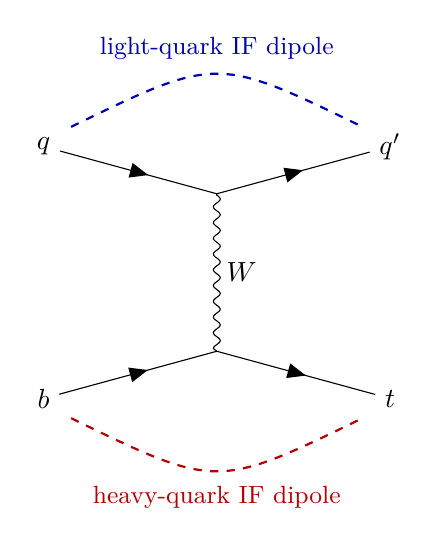
\begin{tikzpicture}[baseline=(current bounding box.center)]
    \begin{feynman}
      \vertex (a) at (0, 1.6) {$q$};
      \vertex (v1) at (2.2, 1.0);
      \vertex (b) at (4.4, 1.6) {$q'$};
      \vertex (c) at (0, -1.6) {$b$};
      \vertex (v2) at (2.2, -1.0);
      \vertex (d) at (4.4, -1.6) {$t$};
      \diagram* {
        (a) -- [fermion] (v1) -- [fermion] (b),
        (v1) -- [boson, edge label=$W$] (v2),
        (c) -- [fermion] (v2) -- [fermion] (d),
      };
    \end{feynman}
    \draw[dashed, thick, blue!70!black] (0.35, 1.85) .. controls (2.2, 2.75) .. (4.05, 1.85);
    \draw[dashed, thick, red!70!black] (0.35, -1.85) .. controls (2.2, -2.75) .. (4.05, -1.85);
    \node[blue!70!black, font=\small] at (2.2, 2.85) {light-quark IF dipole};
    \node[red!70!black, font=\small] at (2.2, -2.85) {heavy-quark IF dipole};
  \end{tikzpicture}
  \caption{Born-level $t$-channel single-top production in the
    five-flavour scheme. Since the $W$ boson is a colour singlet, the
    colour flows from the incoming light quark to the outgoing light
    quark and from the incoming bottom quark to the top quark. The two
    corresponding initial-final colour dipoles are indicated by the
    dashed lines.}
  \label{fig:born}
\end{figure}

\subsection{The local recoil map}
\label{sec:map}

With \code{SpaceShower:dipoleRecoil = on}~\cite{Cabouat:2017rzi},
\pythia describes the gluon emission off an IF dipole as a backward
ISR branching, in which only the final-state end of the dipole, its
colour partner, absorbs the recoil. The same branching also describes
the emission off the final-state end of the dipole, which is therefore
not generated by the FSR, to avoid double counting. Consider a
real-emission configuration with an incoming massless quark with
momentum $p_a$, its outgoing colour partner with momentum $p_f$,
$p_f^2=m_f^2$, which is either the massless light quark ($m_f=0$) or
the top quark ($m_f=m_t$), and the emitted gluon with momentum $k$. We
define the invariants
\begin{equation}
  z=1-\frac{p_f\cdot k}{p_a\cdot(p_f+k)}\,,\qquad
  w=1-z\,,\qquad
  Q^2=2p_a\cdot k\,,\qquad
  \zeta=\frac{p_a\cdot p_f}{p_a\cdot(p_f+k)}\,.
  \label{eq:invariants}
\end{equation}
The momentum fraction $z$ is the backward-evolution variable of the
shower, with evolution variable $p_{\perp\mathrm{evol}}^2=wQ^2$. In
deep-inelastic scattering, $z$ and $\zeta$ coincide with the
variables $x$ and $z_1$ of ref.~\cite{Cabouat:2017rzi}. The local
recoil map projects the real-emission configuration onto the Born
configuration, denoted by tildes,
\begin{equation}
  \tilde p_a=z\,p_a\,,\qquad
  \tilde p_f=p_f+k-w\,p_a\,,
  \label{eq:projection}
\end{equation}
leaving all other momenta, including the other incoming parton,
unchanged. Momentum is conserved, since $p_a-\tilde p_a=p_f+k-\tilde
p_f$, and the definition of $z$ ensures that $\tilde p_f^2=m_f^2$:
the recoil changes the momentum of the colour partner, but preserves
its mass. This map has the same form as the Catani--Seymour map for an
initial-state emitter and a final-state
spectator~\cite{Catani:1996vz,Catani:2002hc}, and the momentum fraction
of the incoming parton changes as $x_a^{\mathrm{B}}=z\,x_a^{\mathrm{R}}$
between the Born and the real-emission configurations. With the dipole
mass $D=2\tilde p_a\cdot\tilde p_f$, one finds
\begin{equation}
  \zeta=1-\frac{zQ^2}{D}\equiv1-\delta\,,
  \label{eq:zeta}
\end{equation}
and the transverse momentum of the emission with respect to the dipole
is
\begin{equation}
  \kt^2=wQ^2\zeta-m_f^2\,\delta^2\,.
  \label{eq:kt}
\end{equation}

The inverse map, from a Born configuration and the radiation
variables $(z,Q^2,\varphi)$ to the real-emission configuration, can be
written in an invariant form. With the light-like vector $n_f=\tilde
p_f-m_f^2\,\tilde p_a/D$, which satisfies $2\tilde p_a\cdot n_f=D$, and
a space-like vector $k_\perp$ orthogonal to $\tilde p_a$ and $n_f$, with
$k_\perp^2=-\kt^2$ and azimuth $\varphi$, the real-emission momenta are
\begin{equation}
  p_a=\frac{\tilde p_a}{z}\,,\qquad
  k=\left[\frac{w}{z}(1-\delta)-\frac{m_f^2}{D}\,\delta\right]\tilde p_a
  +\delta\,n_f+k_\perp\,,\qquad
  p_f=\tilde p_f+\frac{w}{z}\,\tilde p_a-k\,.
  \label{eq:inverse}
\end{equation}
These momenta satisfy $k^2=0$, $p_f^2=m_f^2$ and $2p_a\cdot k=Q^2$. The
physical region is given by
\begin{equation}
  x_a^{\mathrm{B}}<z<1\,,\qquad
  0<\delta<\frac{wD}{wD+z\,m_f^2}\,,
  \label{eq:support}
\end{equation}
where the second condition is equivalent to $\kt^2>0$. This is the
kinematic support of the map. The shower restricts its emissions
further, through its starting scale, its cutoff and, for heavy quarks,
flavour thresholds. Of these, only the starting scale enters the MC
counterterms, see eq.~\eqref{eq:damping} below, while the FKS
subtraction covers the full kinematic support. Including the flux
factors, the real-emission phase space factorises as
\begin{equation}
  \frac{\dd x_a^{\mathrm{R}}\,\dd\PhiR}{2\hat s_{\mathrm{R}}}
  =\frac{\dd x_a^{\mathrm{B}}\,\dd\PhiB}{2\hat s_{\mathrm{B}}}\;
  \frac{\dd z\,\dd Q^2\,\dd\varphi}{32\pi^3}\,,
  \label{eq:measure}
\end{equation}
for both a massless and a massive colour partner, where $\hat
s_{\mathrm{R}}=\hat s_{\mathrm{B}}/z$ are the partonic centre-of-mass
energies squared.

\subsection{The first-emission density}
\label{sec:density}

To first order in $\as$, the probability that the shower emits a gluon
off the IF dipole of a Born configuration with squared matrix element
$B$ is given by the density
\begin{equation}
  \frac{\Dens_0}{B}=\frac{2g_s^2}{zQ^2}\,C_F\,\frac{1+z^2}{1-z}\,,
  \qquad g_s^2=4\pi\as\,,\qquad C_F=\frac{4}{3}\,,
  \label{eq:stockdensity}
\end{equation}
with respect to the measure of eq.~\eqref{eq:measure}, and with the
parton luminosity evaluated for the real-emission configuration. After
the azimuthal integration, this is the familiar backward-evolution
probability $(\as/2\pi)\,(\dd Q^2/Q^2)\,\dd z\,P_{qq}(z)/z$, with
$P_{qq}(z)=C_F(1+z^2)/(1-z)$, where the factor $1/z$ arises from the
ratio $x_a^{\mathrm{R}}f(x_a^{\mathrm{R}})/[x_a^{\mathrm{B}}f(x_a^{\mathrm{B}})]$
of the parton densities in the backward evolution. Hence, the \pythia kernel
for the IF dipoles is the DGLAP kernel of the incoming
quark~\cite{Cabouat:2017rzi}, independently of the momentum fraction
$\zeta$ of the outgoing colour partner. For the channels with an
incoming gluon that splits into a quark that enters the Born process,
the corresponding density is
\begin{equation}
  \frac{\Dens_{g\to q\bar q}}{B}=\frac{2g_s^2}{zQ^2}\,T_R\left[z^2+(1-z)^2\right],
  \qquad T_R=\frac{1}{2}\,,
  \label{eq:gqqdensity}
\end{equation}
which has no soft singularity.

These densities hold for massless incoming quarks, as in the
five-flavour calculation. In its backward evolution, \pythia retains
the masses of incoming charm and bottom quarks: for these, the
numerators of the $q\to qg$ and $g\to q\bar q$ kernels become
$1+z^2-2z(1-z)^2m_q^2/p_{\perp\mathrm{evol}}^2$ and
$z^2+(1-z)^2+2z(1-z)m_q^2/p_{\perp\mathrm{evol}}^2$, respectively, and
close to the quark-mass threshold an incoming bottom or charm quark is
forced to originate from a gluon splitting. These effects are not
included in the MC counterterms. The mass terms decrease as
$m_q^2/p_{\perp\mathrm{evol}}^2$ at large evolution scales, whereas
the forced conversion acts near threshold. We neglect these
power-suppressed effects on infrared-safe observables at hard scales,
as in the usual matching of a massless five-flavour calculation to
the shower.

In FKS subtraction~\cite{Frixione:1995ms,Frixione:1997np,Frederix:2009yq},
the real-emission phase space is partitioned into sectors in which the
gluon can only become collinear to one parton, in this case either to
the incoming quark or to its outgoing colour partner. Since a single
IF dipole of the shower describes both these regions, we use the same
local map, eq.~\eqref{eq:projection}, in both FKS sectors, and we
divide the density between them with
\begin{equation}
  \chi_{\mathrm{I}}=\frac{p_f\cdot k}{p_f\cdot k+p_a\cdot k}\,,\qquad
  \chi_{\mathrm{F}}=\frac{p_a\cdot k}{p_f\cdot k+p_a\cdot k}\,,\qquad
  \chi_{\mathrm{I}}+\chi_{\mathrm{F}}=1\,.
  \label{eq:partition}
\end{equation}
In this way, the density summed over the two sectors is the one of
eq.~\eqref{eq:stockdensity}. Adding independent ISR and FSR
counterterms instead would double count the radiation. The
density of eq.~\eqref{eq:gqqdensity} only contributes to the
initial-state sector.

\subsection{Soft and collinear limits}
\label{sec:limits}

In the collinear limit of the gluon and the incoming quark, $Q^2\to0$
at fixed $z$, one has $\zeta\to1$ and eq.~\eqref{eq:stockdensity}
reproduces the Altarelli--Parisi kernel. Likewise, in the soft limit,
eq.~\eqref{eq:stockdensity} reproduces the eikonal factor of the
dipole,
\begin{equation}
  \frac{\Dens_{0}}{B}\;\to\;2g_s^2C_F\,\frac{p_a\cdot p_f}{(p_a\cdot k)(p_f\cdot k)}\,.
  \label{eq:eikonal}
\end{equation}
There are, however, two limits in which the shower density differs
from QCD.

The first is the limit in which the gluon is collinear to an outgoing
massless quark. With $s_{fk}=2p_f\cdot k=wD/z$, this limit corresponds
to $w\to0$ at fixed $\zeta$, where $\zeta$ becomes the momentum
fraction of the outgoing quark. The coefficient of $2g_s^2/s_{fk}$ is
\begin{equation}
  \text{shower:}\quad\frac{2C_F}{1-\zeta}\,,\qquad\qquad
  \text{QCD:}\quad C_F\,\frac{1+\zeta^2}{1-\zeta}\,.
  \label{eq:finalcollinear}
\end{equation}
The shower thus reproduces the soft-collinear part of the splitting,
but not its hard-collinear part: the difference, $C_F(1+\zeta)$,
multiplies the collinear singularity. This was already noted in
ref.~\cite{Cabouat:2017rzi}, where it was argued that the single IF
description is adequate in view of the good overall agreement with the
DIS matrix elements, and that a separate final-initial description
would require a cumbersome change of variables. For the shower
itself, this is a reasonable approximation. For \mcatnlo matching, it
implies that the difference between the real-emission matrix element
and the MC counterterm has a non-integrable collinear singularity.

The second is the soft limit of the radiation off the heavy-quark
line. For a massive colour partner, the soft current of QCD
gives~\cite{Catani:2002hc}
\begin{equation}
  \frac{\Dens_{\mathrm{QCD,soft}}}{B}
  =2g_s^2C_F\,\frac{p_a\cdot p_f}{(p_a\cdot k)(p_f\cdot k)}
  -g_s^2C_F\,\frac{m_t^2}{(p_f\cdot k)^2}\,.
  \label{eq:softcurrent}
\end{equation}
The second term, the self-eikonal of the top quark, is responsible for
the dead cone around the top quark. It is not generated by the shower:
the top-quark mass enters the local recoil map, eq.~\eqref{eq:inverse},
and its phase-space boundary, eq.~\eqref{eq:support}, but not the
kernel of eq.~\eqref{eq:stockdensity}. Since the difference between
eqs.~\eqref{eq:eikonal} and~\eqref{eq:softcurrent} scales as the inverse
square of the gluon energy, the difference between the real-emission
matrix element and the MC counterterm has a non-integrable soft
singularity. Note that the radiation off the light-quark line has the
correct soft limit.


\section{MC@NLO matching with local recoil}
\label{sec:matching}

\subsection{Phase-space generation}
\label{sec:phasespace}

The MC counterterms must be evaluated with the Born configuration that
the shower would start from. We therefore implement the local recoil
map in the FKS phase-space generation of \mgamc, in both FKS sectors
of each IF dipole, including the inverse map and the massive top quark.
The FKS radiation variables, the energy fraction $\xi$ of the gluon
and the cosine $y$ of its angle with respect to the emitting parton, are
defined in the partonic centre-of-mass frame of the real-emission
configuration. In the initial-state sector, $\xi$ is in general
different from $w$, and solving for the Born configuration at fixed
$\xi$ can have two solutions. We therefore generate the radiation in
terms of $(w,y,\varphi)$, which covers the phase space continuously.
The resulting $\xi$, which enters the prefactors of the real-emission
contribution, and the Jacobian are given in appendix~\ref{app:phasespace}.

The FKS soft counterterms are integrated analytically with a reference
cutoff $\xi_{\mathrm{cut}}$ on the gluon energy
fraction~\cite{Frixione:1995ms}. In the initial-state sector, the soft
subtraction is instead performed in $w$. Near the soft limit,
$\xi=a\,w+\order{w^2}$, where $a$ depends on the direction of the gluon
(see appendix~\ref{app:phasespace}). We distinguish the reference
$w_{\mathrm{ref}}=\xi_{\mathrm{cut}}/a$ from the numerical subtraction
range $h_w=\min(W,\xi_{\mathrm{S,cut}})$, where
$W=1-x_a^{\mathrm{B}}$ is the physical upper limit of $w$ and
$\xi_{\mathrm{S,cut}}$ is the independently chosen subtraction
parameter. At fixed Born configuration and gluon direction, let
$F(w)/w$ denote the soft-singular density, with $F_0=F(0)$. In
$4-2\epsilon$ dimensions,
\begin{align}
 a^{-2\epsilon}\int_0^W\!\dd w\,\frac{F(w)}{w^{1+2\epsilon}}
 ={}&-\frac{F_0}{2\epsilon}+F_0\log\xi_{\mathrm{cut}}
 +\int_0^W\!\frac{\dd w}{w}
       \left[F(w)-F_0\,\Theta(h_w-w)\right]\nonumber\\
 &+F_0\log\frac{a h_w}{\xi_{\mathrm{cut}}}
 +\order{\epsilon}\,.
 \label{eq:softreference}
\end{align}
The last term is retained in the finite soft counterevent. The
reference $w_{\mathrm{ref}}$ is not clipped at $W$: if
$w_{\mathrm{ref}}>W$ and $h_w=W$, this term is
$-F_0\log(w_{\mathrm{ref}}/W)$. Thus the standard integrated soft
counterterms remain valid even when the reference exceeds the
physical range. In the implementation, this finite term is sampled
uniformly over $0<w<h_w$, with density
$F_0\log(a h_w/\xi_{\mathrm{cut}})/h_w$. It belongs only to the FKS
subtraction, not to the G-function replacements. Since $a\to1$ in
the collinear limit of the gluon and the incoming quark, no change
of the integrated collinear counterterms or of the PDF counterterms
is required.

The $\clS$ events receive the MC counterterms and the FKS soft and
collinear counterterms of all FKS sectors with the same Born
configuration. In the local matching, we sum explicitly over all FKS
sectors and all Born colour dipoles at each phase-space point. Since
the different sectors use different frames and energy variables, we
generate their soft limits from a single gluon direction in the Born
centre-of-mass frame and with the same physical gluon energy, see
appendix~\ref{app:phasespace}. Otherwise, the soft limits of the
contributions to an $\clS$ event would be evaluated at different
configurations, which leaves a finite mismatch.

\subsection{MC counterterms with G functions}
\label{sec:Gfunctions}

Schematically, and suppressing the sums over FKS sectors and colour
dipoles, the $\clS$- and $\clH$-event contributions of \mcatnlo
are~\cite{Frixione:2002ik,Alwall:2014hca}
\begin{equation}
  \clS:\quad B+V+I+\int\dd\Phi_{\mathrm{rad}}\left(\Dens_{\mathrm{MC}}-C\right),\qquad\qquad
  \clH:\quad R-\Dens_{\mathrm{MC}}\,,
  \label{eq:SH}
\end{equation}
where $R$ and $V$ are the real-emission and virtual contributions,
$C$ the FKS counterterms and $I$ their integrated counterparts, and
$\Dens_{\mathrm{MC}}$ the MC counterterm. Both $\clS$ and $\clH$
contributions are finite only if $\Dens_{\mathrm{MC}}$ has the same soft and
collinear singularities as $R$. As discussed in
section~\ref{sec:limits}, this is not the case for
$\Dens_{\mathrm{MC}}=\Dens_0$. In \mgamc, the mismatch in the
soft limit, which is due to the angular pattern of soft radiation in
the \pythia and \textsc{Herwig} showers, is solved by replacing the MC
counterterm by the soft limit of the real-emission matrix element in
a region around the soft limit, through a G
function~\cite{Alwall:2014hca}. We extend this to the hard-collinear
limit of the outgoing quark.

Let $S$, $C_{\mathrm{coll}}$ and $SC$ denote the soft, collinear and
soft-collinear FKS counterterms of a sector, including their sector
functions. We define the smooth profile
\begin{equation}
  g_h(v)=\begin{cases}
    0\,, & v\le0\,,\\[2pt]
    \dfrac{u^2}{u^2+(1-u)^2}\,,\quad u=v/h\,, & 0<v<h\,,\\[8pt]
    1\,, & v\ge h\,,
  \end{cases}
  \label{eq:profile}
\end{equation}
with width $h$, and the MC counterterm
\begin{equation}
  \Dens_G=d(q)\Big\{g_h(w)\,\Dens_0+\left[1-g_h(w)\right]
  \Big[S+\left[1-g_h(1-y)\right]\left(C_{\mathrm{coll}}-SC\right)\Big]\Big\}.
  \label{eq:DG}
\end{equation}
In the notation of ref.~\cite{Alwall:2014hca}, $1-g_h$ plays the role
of the G function. A similar combination of soft, collinear and
soft-collinear replacements, with independent damping functions of a
soft and of an angular variable, was used for heavy-flavour production
in ref.~\cite{Frixione:2003ei} (see eq.~(B.43) there). Here, the
replacement is restricted to the region $w<h$, and the same width $h$
is used in the angular profile $g_h(1-y)$, so that $h$ is the only
parameter of the prescription. The variable $w=1-z$ vanishes both for
soft gluons and for gluons collinear to the outgoing quark at finite
$\zeta$, so that $g_h(w)$ removes both mismatches of
section~\ref{sec:limits}; a profile in the gluon energy would leave the
collinear mismatch. Since $2p_f\cdot k=wD/z$, the region $w<h$
corresponds to $(p_f+k)^2-m_f^2<h\,D/z$: the invariant mass of the
gluon and the colour partner must be close to the mass of the latter,
in units of the dipole invariant $D$. Hence, $w<h$ does not correspond
to a fixed energy or transverse momentum of the gluon; for the
light-quark line with $h=0.01$, for example, it corresponds to
$m(f,k)<0.1\sqrt{D/z}$. The angular profile $g_h(1-y)$, with $y$ the
FKS angular variable of the sector, restricts the collinear
counterterm to the vicinity of the collinear limit. This term is
needed since the soft counterterm alone
does not have the correct collinear limit, so that a pure soft
replacement would in turn spoil the collinear limit in the transition
region; the subtraction of the soft-collinear counterterm $SC$ avoids
double counting. The factor
\begin{equation}
  d(q)=1-g_1\!\left(\frac{q-\mu_{\min}}{\mu_{\max}-\mu_{\min}}\right),
  \label{eq:damping}
\end{equation}
where $\mu_{\min}$ and $\mu_{\max}$ delimit the range of shower
starting scales of the Born dipole, implements the smooth dependence on
the shower starting scale~\cite{Alwall:2014hca}. It is evaluated with
the evolution variable of the shower, $q^2=p_{\perp\mathrm{evol}}^2=wQ^2$,
and it multiplies the replacement terms as well, since otherwise the
replacement would be active above the shower starting scale. The
density of eq.~\eqref{eq:gqqdensity} has the correct collinear limit
and needs no replacement. We use $h=0.01$ as default value.

The difference between the actual first emission of the shower,
$\Dens_{\mathrm{PS}}=d(q)\,\Dens_0$, and the MC counterterm leads to a
mismatch in the expansion of an infrared-safe observable $O$,
\begin{equation}
  \delta\sigma[O]=\int\dd\PhiR\,\left(\Dens_{\mathrm{PS}}-\Dens_G\right)
  \left[O(\PhiR)-O(\PhiB)\right],
  \label{eq:mismatch}
\end{equation}
which is restricted to the region $w<h$ and vanishes as $h\to0$.
These are the same power-suppressed effects as discussed in
ref.~\cite{Alwall:2014hca} for the soft G functions. However, at
finite $h$, this mismatch is not suppressed by an additional power of
$\as$, and the dependence on $h$ should be considered a matching
uncertainty. A smaller $h$ reduces this uncertainty, at the price of
larger cancellations between the event weights.

\subsection{Corrections to the Pythia8 kernel}
\label{sec:patches}

As noted in ref.~\cite{Alwall:2014hca}, for a shower with the correct
soft behaviour, the MC counterterms can be constructed without G
functions. For the $t$-channel single-top process, this requires two
corrections of the IF kernel of \pythia, which we have implemented in
\textsc{Pythia}~8.318 as optional weights in the veto step of the backward
evolution.

The first replaces the numerator of the kernel for an incoming quark
that emits a gluon, with an outgoing quark or antiquark as colour
partner,
\begin{equation}
  C_F\frac{1+z^2}{1-z}\;\longrightarrow\;C_F\frac{z^2+\zeta^2}{1-z}\,,
  \qquad\text{i.e.,}\qquad
  r_q=\frac{z^2+\zeta^2}{1+z^2}\,.
  \label{eq:rq}
\end{equation}
In the physical region, $0\le\zeta\le1$ and thus $0\le r_q\le1$. In the
soft limit and in the collinear limit of the incoming quark, $r_q\to1$,
whereas in the collinear limit of the outgoing quark, $z\to1$, the
numerator becomes $1+\zeta^2$, as required by
eq.~\eqref{eq:finalcollinear}. The numerator $z^2+\zeta^2$ is the one
of the singular part of the matrix element for DIS, cf.\
ref.~\cite{Cabouat:2017rzi}. Away from the singular limits, however,
$r_q$ is a choice, which modifies the finite part of the emission rate,
also on the heavy-quark line.

The second multiplies the kernel for an incoming quark that emits a
gluon, with the top quark as colour partner, by
\begin{equation}
  r_t=1-\frac{m_t^2\,(p_a\cdot k)}{2(p_a\cdot p_f)(p_f\cdot k)}
     =1-\frac{m_t^2z^2Q^2}{w\,\zeta D^2}
     =\frac{\kt^2}{wQ^2\zeta}\,.
  \label{eq:rt}
\end{equation}
Multiplying the eikonal factor of eq.~\eqref{eq:eikonal} by $r_t$ gives
exactly the massive soft current of eq.~\eqref{eq:softcurrent}. In the
rest frame of the top quark, $r_t=(1+\cos\theta_{ak})/2$, with
$\theta_{ak}$ the angle between the incoming quark and the gluon; hence
$0\le r_t\le1$. In the collinear limit of the incoming quark, $r_t\to1$.
As for $r_q$, the extension of $r_t$ away from the soft limit is a
choice, which modifies the finite part of the emission rate. Since the
corrections are applied before an emission is accepted, they
change the Sudakov form factor consistently with the emission rate.
Since $r_q$ and $r_t$ are bounded by one, the overestimates of the
trial emissions remain valid. Both corrections are switched off by
default; the implementation is described in appendix~\ref{app:pythia}.

With both corrections, the MC counterterm for the heavy-quark line is
\begin{equation}
  \frac{\Dens_2}{B}=\frac{2g_s^2}{zQ^2}\,C_F\,\frac{z^2+\zeta^2}{1-z}\,r_t\,,
  \label{eq:D2}
\end{equation}
and the one for the light-quark line is the same without $r_t$. For
massless incoming quarks, these have the correct soft and collinear
limits, so the MC counterterms can be used without G functions, i.e.,
$\Dens_{\mathrm{MC}}=d(q)\,\Dens_2$. Note that the partition of
eq.~\eqref{eq:partition} differs from the partition of the phase space
by the FKS sector functions. In a given FKS sector, the soft limit of
the real-emission matrix element is given by the soft current of the
full Born process, including the radiation off the other colour line,
whereas the MC counterterm assigned to that sector only contains a
fraction of the density of one dipole. Without G functions, the
collinear singularities therefore cancel sector by sector, but the soft
singularities cancel only in the sum over all FKS sectors and colour
dipoles with the same Born configuration. This is one of the reasons
for the explicit sums and the common soft configuration of
section~\ref{sec:phasespace}. With G functions, instead, the MC
counterterm of each sector tends to the FKS soft counterterm of that
sector in the soft limit. We give the explicit sums below.

With only the $r_q$ correction, the outgoing-quark collinear limit is
correct, but the soft limit of the heavy-quark line is not. In that
case, we use eq.~\eqref{eq:DG} with the corrected density, but with
the profile $g_h(\xi)$ in the energy fraction of the gluon in the
partonic centre-of-mass frame of the real-emission configuration,
which is independent of the FKS sector, instead of $g_h(w)$. In this
case, the replacement is thus active for gluon energies below
$h\sqrt{\hat s_{\mathrm{R}}}/2$ in that frame.

The $r_t$ correction applies to the current colour connection between
an incoming quark and the top quark. Hence it also applies to
subsequent emissions, as long as this connection is intact, for
example after an emission off the light-quark line. After a gluon
emission off the heavy-quark line, the top quark forms a final-final
dipole with the gluon, which is not modified: \pythia already includes
the mass effects of the top quark in its FSR~\cite{Norrbin:2000uu}, as
well as an additional suppression for a gluon that recoils against a
massive quark~\cite{Bierlich:2022pfr}. Configurations in which a top quark is
colour-connected to an incoming gluon, for example after a backward
$g\to b\bar b$ splitting, are not modified either. The corrections
change the hard-emission rates and the shower beyond the first
emission, and we make no claim about the logarithmic accuracy of the
modified shower. Matrix-element corrections are switched off in all
our simulations, as is usually recommended for \mcatnlo matching (see
refs.~\cite{Frixione:2023hwz,Frederix:2024psm} for a discussion); in
any case, they would have to be redefined with respect to the modified
emission rates.

\subsection{Sector and dipole sums}
\label{sec:sectorsums}

Let $\beta=(d,r)$ label a native radiation history, including its
flavours, with Born colour line $d$ (light or heavy) and FKS orientation
$r=\mathrm{I},\mathrm{F}$. For gluon radiation there are four such
histories; the $g\to q\bar q$ histories have only an initial-state
orientation. Let $F_\beta(\PhiR)$ be the FKS sector function, normalised
so that $\sum_\beta F_\beta=1$ for a fixed real channel, and let
$\Pi_\beta\PhiR$ be its local Born projection. The two orientations
of one dipole have the same projection, while projections onto
different dipoles generally differ away from the singular limits.

We include parton luminosities in the densities in this subsection.
Writing $B$ without luminosities in the next equation only, the raw
MC density assigned to history $\beta$ is
\begin{equation}
 A_\beta(\PhiR)=\chi_r(\PhiR)\,
 B(\Pi_\beta\PhiR)\,
 {\cal L}^{\mathrm{R}}_\beta\,
 \left(\frac{\Dens}{B}\right)_\beta,
 \qquad
 {\cal L}^{\mathrm{R}}_\beta=
 f_{a_\beta^{\mathrm{R}}}(x_{a,\beta}^{\mathrm{B}}/z_\beta,\mu_F)
 f_b(x_b^{\mathrm{B}},\mu_F)\,.
 \label{eq:nativeMC}
\end{equation}
Here $a$ is the incoming end of that dipole, $b$ is the other beam,
$a_\beta^{\mathrm{R}}$ is its real-channel flavour, and the hard
coupling and factorisation scales are evaluated in that history.
The density $\Dens/B$ is eq.~\eqref{eq:stockdensity}, or its patched
counterpart, before multiplication by $\chi_r$, the starting-scale
damping or a G function. Both orientations use the real luminosity
shown above, including the final-state FKS orientation: the shower
emission is always generated by backward evolution. The $1/z_\beta$
is already in $\Dens/B$ and is not inserted again in the luminosity.
For $g\to q\bar q$, use eq.~\eqref{eq:gqqdensity} and no $\chi_r$.
There is no extra factor $F_\beta$ multiplying $A_\beta$.

Let $S_\beta$, $C_{\mathrm{coll},\beta}$ and $SC_\beta$ be the exact
FKS endpoint densities, including their FKS sector functions, native
endpoint Jacobians and endpoint luminosities, pulled back to the
real-emission measure of history $\beta$. In particular, a replacement
term retains its counterevent luminosity rather than the real
luminosity of eq.~\eqref{eq:nativeMC}. We write
$c_\beta=g_h(1-y_\beta)$ and $d_\beta=d(q_\beta)$. Taking
$g_\beta=g_h(w_\beta)$ for \loc and
$g_\beta=g_h(\xi)$ for \locq, the complete MC density is
\begin{equation}
 M_\beta=d_\beta\left\{
 g_\beta A_\beta+(1-g_\beta)
 \left[S_\beta+(1-c_\beta)
 (C_{\mathrm{coll},\beta}-SC_\beta)\right]\right\}.
 \label{eq:sectorMC}
\end{equation}
For \locqt, $M_\beta=d_\beta A_\beta$; the conversion histories also
need no G replacement. For a massive final-state emitter there is no
collinear or soft-collinear endpoint term. All endpoint measure
ratios in eq.~\eqref{eq:sectorMC} are those of the same native map;
they cannot be replaced by the measure of an outer sector.

At fixed Born configuration, the $\clS$ weight is
\begin{equation}
 \dd\sigma_{\clS}=\dd\PhiB\left[
 B+V+I+\sum_\beta\int\dd\rho_\beta
 \left(J_\beta M_\beta-C^{\mathrm{FKS}}_\beta\right)\right],
 \label{eq:Sresolved}
\end{equation}
where $\rho_\beta$ denotes the three native radiation coordinates,
$\PhiR=T_\beta(\PhiB,\rho_\beta)$ is the forward local map,
$J_\beta\,\dd\PhiB\,\dd\rho_\beta=\dd\PhiR$, and
$C^{\mathrm{FKS}}_\beta$ includes the ordinary subtraction cutoffs,
endpoint measures and the finite term of eq.~\eqref{eq:softreference}.
The phase-space measures here also include the incoming momentum
fractions and flux factors. The Born, virtual and integrated
contributions are included once. The radiation terms are summed at
the common Born point and common soft momentum described in
section~\ref{sec:phasespace}, before taking absolute weights for event
generation.

For $\clH$ events, an outer sector $\alpha$ generates a real point,
and its weight is
\begin{align}
 \widehat H_\alpha(\PhiR)
 &=F_\alpha(\PhiR)\sum_\beta
 \left[F_\beta(\PhiR)R(\PhiR)-M_\beta(\PhiR)\right]\nonumber\\
 &=F_\alpha(\PhiR)\left[R(\PhiR)-\sum_\beta M_\beta(\PhiR)\right].
 \label{eq:Hresolved}
\end{align}
Every native history is reconstructed from that same real point and
uses its own $\Pi_\beta$, luminosities and shower-scale bounds. If a
native summand has already been multiplied by its real Jacobian
$J_\beta$, it is converted to the outer integration measure by
$F_\alpha J_\alpha/J_\beta$. This conversion retains the endpoint to
real measure ratios inside $M_\beta$. The sum is formed before
unweighting, and the emitted event has the common real momenta; the
outer sector supplies its event colour and shower-scale assignment.
Thus $F_\beta R-M_\beta$ is an intermediate summand, not an
independently generated hard-event contribution. Summing
eq.~\eqref{eq:Hresolved} over $\alpha$ gives
$R-\sum_\beta M_\beta$, and the integrated MC terms cancel those in
eq.~\eqref{eq:Sresolved} for an observable that is constant on phase
space.

For completeness, consider the soft limit without G functions. Let
$E_d$ be the exact soft density of Born line $d$, including its Born
matrix element and luminosity, and let $R_{\mathrm{s}}=E_\ell+E_h$.
The two-patch kernel obeys
\begin{equation}
 M_{(d,r)}\longrightarrow\chi_r E_d,\qquad
 F_\beta R-M_\beta\longrightarrow
 F_\beta R_{\mathrm{s}}-\chi_r E_d,\qquad
 \sum_\beta\left(F_\beta R_{\mathrm{s}}-\chi_r E_d\right)=0\,.
 \label{eq:softsum}
\end{equation}
Here $d_\beta\to1$, all Born projections approach the same Born
point, and $\sum_r\chi_r=1$ for each line. This proves the soft
cancellation in the hard-event sum and, with the common soft
coordinates, in the $\clS$ integrand. With G functions,
$M_\beta\to S_\beta$ instead, so the soft cancellation is already
sector by sector. In a massless collinear limit the corresponding
$F_\beta\to1$ and $\chi_r\to1$, while the complementary
orientation vanishes. The corrected kernels give the appropriate
Altarelli--Parisi limit, or the G replacement supplies it, so
$M_\beta$ and $F_\beta R$ have the same collinear singularity.
The incoming-gluon conversion obeys the same statement with
eq.~\eqref{eq:gqqdensity}. No collinear limit is required for the
massive top quark.

\subsection{The four predictions}
\label{sec:predictions}

\begin{table}[t]
  \centering
  \begin{tabular}{@{}llll@{}}
    \toprule
    Prediction & Recoil & IF kernel numerator & MC counterterm\\
    \midrule
    \glob & global & standard & default~\cite{Alwall:2014hca}\\
    \loc & local & $1+z^2$ & $\Dens_G$ with $g_h(w)$\\
    \locq & local & $z^2+\zeta^2$ & $\Dens_G$ with $g_h(\xi)$\\
    \locqt & local & $(z^2+\zeta^2)\,r_t$ & $d(q)\,\Dens_2$\\
    \bottomrule
  \end{tabular}
  \caption{The four \mcatnlo predictions: the recoil scheme of
    \pythia, the numerator of its IF kernel, which multiplies
    $C_F/(1-z)$, and the MC counterterms. The numerator is given for
    the heavy-quark line; the $r_t$ factor does not apply to the
    light-quark line. The G-function width is $h=0.01$; the \locqt
    prediction needs no G functions.}
  \label{tab:predictions}
\end{table}

The four predictions that we compare are summarised in
table~\ref{tab:predictions}. The \glob prediction is the default of
\mgamc, with the global recoil schemes of \pythia. The \loc, \locq and
\locqt predictions use \pythia with local recoil, without and with the
kernel corrections of section~\ref{sec:patches}, and the corresponding
MC counterterms. For the latter two, we use private builds of
\textsc{Pythia}~8.318 with the corrections switched on; with the corrections
switched off, these builds reproduce the unmodified \pythia shower.
Apart from the phase-space parametrisation and the MC counterterms,
the four predictions use the same short-distance cross sections, the
same parameters and the same functional prescription for the shower
starting scales. The numerical values of the latter can nevertheless
differ between the predictions, since they depend on the Born
configuration and the colour dipole, and thus on the recoil map.

\subsection{Validation}
\label{sec:validation}

We have tested the implementation of the local recoil map for both
beams, for quarks and antiquarks and for a massless and a massive
colour partner: the closure of the forward and inverse maps, the
preservation of masses and of the momenta not involved in the
emission, the boundaries of the phase space and the Bjorken fractions.
The phase-space measure has been compared with the numerical
determinant of the Cartesian phase-space parametrisation, and the
finite soft term of section~\ref{sec:phasespace} with the dimensionally
regulated energy integral.

\begin{table}[t]
  \centering
  \begin{tabular}{@{}lcrrr@{}}
    \toprule
    FKS map & $(\xi_{\mathrm{S,cut}},\delta_{\mathrm S})$ & Seed & $\sigma_{\mathrm{NLO}}$ [pb] & $p_i$\\
    \midrule
    default & $(0.5,1)$ & 710101 & $132.039\pm0.088$ & $-0.52$\\
    & & 710102 & $132.093\pm0.079$ & $+0.29$\\
    & & 710103 & $132.094\pm0.096$ & $+0.22$\\
    & & combined & $132.076\pm0.050$ & ---\\
    \midrule
    default & $(0.25,0.5)$ & 710201 & $132.049\pm0.103$ & $+0.03$\\
    & & 710202 & $132.069\pm0.071$ & $+0.44$\\
    & & 710203 & $132.009\pm0.090$ & $-0.50$\\
    & & combined & $132.047\pm0.049$ & ---\\
    \midrule
    local & $(0.5,1)$ & 710301 & $132.283\pm0.121$ & $+1.79$\\
    & & 710302 & $132.016\pm0.096$ & $-1.08$\\
    & & 710303 & $132.056\pm0.100$ & $-0.51$\\
    & & combined & $132.096\pm0.060$ & ---\\
    \midrule
    local & $(0.25,0.5)$ & 710401 & $132.051\pm0.090$ & $+0.52$\\
    & & 710402 & $131.800\pm0.133$ & $-1.87$\\
    & & 710403 & $132.140\pm0.122$ & $+1.18$\\
    & & combined & $132.018\pm0.064$ & ---\\
    \bottomrule
  \end{tabular}
  \caption{Fixed-order NLO cross sections for $pp\to t+j+X$ at
    $\sqrt{s}=13\TeV$, with the production setup of
    section~\ref{sec:setup} and no generation cuts. The parameters
    $\xi_{\mathrm{S,cut}}$ and $\delta_{\mathrm S}$ delimit the numerical
    subtraction ranges; the analytic reference parameters are kept
    fixed. Each pair of map and cutoffs uses three independent seeds.
    Combined results are inverse-variance weighted means $\bar\sigma$,
    with uncertainty $\delta\bar\sigma$. The seed pulls are
    $p_i=(\sigma_i-\bar\sigma)/\sqrt{\delta\sigma_i^2-\delta\bar\sigma^2}$,
    accounting for the contribution of seed $i$ to the mean. All
    uncertainties are statistical.}
  \label{tab:fixedorder}
\end{table}

Since the phase-space parametrisation does not change the NLO cross
section, the fixed-order results with the default FKS maps and with
the local map must agree. Table~\ref{tab:fixedorder} shows the total
cross sections from twelve integrations with the production setup,
with a requested relative accuracy of $0.1\%$ per seed. Neither MC
counterterms nor showers enter this comparison. The three seeds in
each group give $\chi^2=0.27$, $0.28$, $3.27$ and $3.83$ for two
degrees of freedom, in table order, with corresponding $p$ values
between $0.15$ and $0.88$.

For $(\xi_{\mathrm{S,cut}},\delta_{\mathrm S})=(0.5,1)$ and
$(0.25,0.5)$, the local-minus-default differences of the combined
results are $0.020\pm0.078\pb$ and $-0.029\pm0.080\pb$, respectively,
corresponding to pulls of $+0.26$ and $-0.36$. Changing the cutoffs
from the first to the second setting gives pulls of $-0.41$ for the
default map and $-0.89$ for the local map. These pulls use independent
sample errors added in quadrature. Thus, the inclusive NLO cross
section is independent of the recoil map and of the numerical
subtraction ranges within the statistical precision of the test,
about $0.06\%$ on the difference of the two maps.
% Completed campaign F; full-precision results and checks are archived in
% fixed_order_results.json. Run definitions are in proposed_runs.csv.

For all subprocesses, the real-emission matrix elements approach the
FKS counterterms as well as the MC counterterms in the soft and
collinear limits, as verified with the standard tests of \mgamc, and
the infrared poles of the virtual corrections cancel.

The shower density of eq.~\eqref{eq:stockdensity} has been compared
with the unmodified \textsc{Pythia}~8.318. For 1200 accepted first emissions,
for both beams and for quarks and antiquarks, we have verified the
recoil map and the selection of the colour partner, and for 100 of
them we have verified that the density of the MC counterterms agrees
with the one of the shower. The same comparisons for 100 accepted
emissions have been done for each of the two shower modifications,
together with the bounds of $r_q$ and $r_t$, and we have verified that
the modified builds with the corrections switched off reproduce the
unmodified shower exactly.

Finally, we have generated MC@NLO samples for the \loc prediction with
the G-function widths $h=0.005$, $0.01$ and $0.02$, with the earlier
validation cut $\pT(j)>10\GeV$ at generation level. The total cross sections are
$132.1\pm2.5\pb$, $134.7\pm1.6\pb$ and $134.9\pm1.7\pb$, respectively,
and the fractions of negative-weight events among the first 1000 events
are $24.7\%$, $26.7\%$ and $23.8\%$. These samples are statistically
compatible and the event weights are finite. However, since
$O(\PhiR)=O(\PhiB)$ for the total cross section, the mismatch of
eq.~\eqref{eq:mismatch} does not contribute to it: these samples test
the stability of the integration, but not the size of the mismatch,
which requires differential distributions. \todo{Differential
  variations of $h$ for the \loc and \locq predictions, with the
  production setup and statistics, for $\pT(t+j_1)$ including its first
  bins, $z^*_{j_2}$, the gap fraction at small $Q_0$, a Born observable,
  and the TAG and GAP acceptances.}
% Proposed runs: G in TODO_runs.txt and proposed_runs.csv.


\section{Results for \texorpdfstring{$t$}{t}-channel single-top production at the LHC}
\label{sec:results}

\paragraph{Status of the numerical results.}
The MC@NLO samples underlying the tables and distributions below require
regeneration. An inclusive normalization check identified an uninitialized
momentum for the coloured mother of the final clustering vertex, which
gave inconsistent shower damping scales in the S and H contributions.
The initialization has been corrected and subtraction closure restored.
The existing MC@NLO numbers and their phenomenological interpretation
are retained here as a record of the earlier samples, pending replacement.
The fixed-order validation and the POWHEG sample are unaffected.

\subsection{Setup}
\label{sec:setup}

We consider $pp$ collisions at $\sqrt{s}=13\TeV$, with $m_t=173\GeV$,
the NNPDF2.3 NLO parton densities~\cite{Ball:2012cx} and
\begin{equation}
  \mu_R=\mu_F=\frac{H_T}{2}\,,\qquad
  H_T=\sum_{i\in\mathrm{final}}\sqrt{m_i^2+p_{T,i}^2}\,,
  \label{eq:scales}
\end{equation}
where the sum runs over all final-state particles of the hard
process. No cuts are applied at generation level. For each of the four
predictions of table~\ref{tab:predictions}, we generate $10^6$
unweighted events with \mgamc and shower them with \textsc{Pythia}~8.318.
Only top quarks are generated, i.e., no antitop quarks.

\begin{table}[t]
  \centering
  \begin{tabular}{@{}lcc@{}}
    \toprule
    \pythia setting & \glob & local recoil\\
    \midrule
    \code{SpaceShower:dipoleRecoil} & off & on\\
    \code{TimeShower:globalRecoil} & on & off\\
    \midrule
    QCD ISR and FSR & \multicolumn{2}{c}{on}\\
    QED and weak showers & \multicolumn{2}{c}{off}\\
    MPI, beam remnants, primordial $k_T$ & \multicolumn{2}{c}{off}\\
    colour reconnection, hadronisation & \multicolumn{2}{c}{off}\\
    top-quark decay & \multicolumn{2}{c}{off}\\
    matrix-element corrections & \multicolumn{2}{c}{off}\\
    $\as(M_Z)$ in the shower & \multicolumn{2}{c}{0.118, one-loop running}\\
    shower PDFs (\code{PDF:pSet}) & \multicolumn{2}{c}{15 (NNPDF2.3 QCD+QED NLO)}\\
    \code{SpaceShower:pT0Ref} & \multicolumn{2}{c}{0}\\
    \code{SpaceShower/TimeShower:pTmaxMatch} & \multicolumn{2}{c}{1}\\
    \code{TimeShower:weightGluonToQuark} & \multicolumn{2}{c}{1}\\
    \code{TimeShower:recoilDeadCone} & \multicolumn{2}{c}{on}\\
    \bottomrule
  \end{tabular}
  \caption{The settings of \pythia that are relevant for this study,
    for the \glob prediction and for the three local-recoil
    predictions.}
  \label{tab:settings}
\end{table}

The settings of \pythia are listed in table~\ref{tab:settings}. We
switch off all effects that are not related to the perturbative QCD
shower, and we keep the top quark stable. The regularisation of the
ISR at small transverse momenta, \code{SpaceShower:pT0Ref}, is
switched off, while the shower cutoff remains active. The \glob
prediction uses the global-recoil settings of the default \mgamc
interface, in which the recoil of the first FSR emission off $\clS$
events is shared by all final-state partons and the recoil of an ISR
emission is taken by the whole final state. The three local-recoil
predictions use \code{SpaceShower:dipoleRecoil = on}, which, as
required, is not combined with global recoil for the FSR. The shower
starting scales and their smooth damping are the default ones of
\mgamc.\footnote{With global recoil, the event record of \pythia
  contains many copies of the recoiling partons, and it can exceed
  the default size of 4000 entries of the \code{HEPEVT} common block
  through which the events are passed to the Fortran analysis. In
  that case, the record is truncated and the top quark can be lost.
  We have therefore increased this size to $10^5$ entries, and the
  analysis refuses records that reach this size.}

\subsection{Analysis}
\label{sec:analysis}

Final-state partons, apart from the top quark, are clustered into jets
with the anti-$k_T$ algorithm~\cite{Cacciari:2008gp} with $R=0.4$, as
implemented in \textsc{FastJet}~\cite{Cacciari:2011ma}. Jets are
required to have $\pT>20\GeV$ and $|y|<4.5$, and they are ordered in
transverse momentum. The leading jet $j_1$ is a proxy for the
spectator jet; it is not identified by flavour or by its origin. In
particular, $j_1$ can originate from additional radiation, for example
from the antiquark of an initial-state gluon splitting, rather than from
the outgoing light quark of the Born process, which can also lead to
migrations between the selections. We consider three selections:
\begin{itemize}
\item ALL: all events;
\item TAG: events with $\pT(j_1)>30\GeV$;
\item GAP: events in TAG with, in addition, $|y(t)-y(j_1)|>3$ and
  $m(t,j_1)>500\GeV$.
\end{itemize}
The GAP selection is similar to typical VBF selections, with the top
quark taking the place of one of the tagging jets; it serves as a
diagnostic of the radiation pattern, rather than as an experimental
fiducial region. To study the
position of the second jet $j_2$ with respect to the top quark and the
leading jet, we use the oriented Zeppenfeld variable
\begin{equation}
  z^*_{j_2}=s\,\frac{y(j_2)-\frac{1}{2}\left[y(t)+y(j_1)\right]}{|y(j_1)-y(t)|}\,,
  \qquad s=\mathrm{sign}\left[y(j_1)-y(t)\right],
  \label{eq:zstar}
\end{equation}
for which the top quark is at $z^*=-1/2$ and the leading jet at
$z^*=+1/2$, independently of their orientation. For this variable, we
require $|y(j_1)-y(t)|>1$, in addition to the TAG or GAP selections.
In the same way, we use the oriented rapidity differences
$s\,[y(j_2)-y(t)]$ and $s\,[y(j_2)-y(j_1)]$. Finally, we define the
gap fraction $f_{\mathrm{gap}}(Q_0)$ as the fraction of events in a
selection that have no jet other than $j_1$ with $\pT\ge Q_0$ in the
rapidity interval between the top quark and the leading jet.

All uncertainties shown are statistical. The \mcatnlo event weights
are signed, and their uncertainties are computed from the sum of the
squared weights. For the gap fraction, the correlation between the
numerator and the denominator is taken into account. We do not
consider scale or PDF uncertainties, nor uncertainties related to the
matching, such as the shower starting scale or the G-function width.
The differences between the predictions shown below therefore
establish the effects of the recoil scheme and of the kernel
corrections in this setup, but not the uncertainties of the
predictions. \todo{Variations of the shower starting scale and of the
  renormalisation and factorisation scales (and of the G-function
  width, see section~\ref{sec:validation}) for the central observables;
  a comparison with POWHEG+\pythia with dipole recoil.}
% Proposed runs: S and W in TODO_runs.txt and proposed_runs.csv.
% W setup: ../pp_tj_powheg/README.powheg; production not yet run.

\subsection{Rates and event weights}
\label{sec:rates}

\begin{table}[t]
  \centering
  \begin{tabular}{@{}lcccc@{}}
    \toprule
    & \glob & \loc & \locq & \locqt\\
    \midrule
    ALL [pb] & $138.45\pm0.34$ & $138.42\pm0.29$ & $137.51\pm0.25$ & $138.28\pm0.23$\\
    TAG [pb] & $104.59\pm0.29$ & $102.86\pm0.23$ & $102.20\pm0.20$ & $102.78\pm0.18$\\
    GAP [pb] & $19.10\pm0.13$ & $18.81\pm0.10$ & $18.70\pm0.09$ & $18.75\pm0.08$\\
    \midrule
    TAG, $N_{\mathrm{jets}}\ge2$ [pb] & $51.65\pm0.20$ & $49.15\pm0.15$ & $48.65\pm0.13$ & $47.22\pm0.12$\\
    GAP, $N_{\mathrm{jets}}\ge2$ [pb] & $8.11\pm0.08$ & $7.21\pm0.06$ & $7.03\pm0.05$ & $6.77\pm0.05$\\
    TAG, $|z^*_{j_2}|<1/2$ [pb] & $10.09\pm0.10$ & $8.17\pm0.06$ & $8.01\pm0.05$ & $7.91\pm0.05$\\
    GAP, $|z^*_{j_2}|<1/2$ [pb] & $3.43\pm0.06$ & $2.46\pm0.03$ & $2.38\pm0.03$ & $2.37\pm0.03$\\
    \midrule
    $N_{\mathrm{eff}}/N$ & $0.164$ & $0.226$ & $0.292$ & $0.353$\\
    negative-weight fraction & $29.8\%$ & $26.2\%$ & $23.0\%$ & $20.3\%$\\
    \bottomrule
  \end{tabular}
  \caption{Cross sections in the three selections, in the selections
    with at least two jets, and with the second jet in the rapidity
    interval between the top quark and the leading jet; for the latter,
    $|y(j_1)-y(t)|>1$ is required in addition, which only affects the
    TAG selection. The last two rows give the effective sample size of
    the total cross section relative to the number of events, and the
    fraction of negative-weight events inferred from it. The
    uncertainties are the statistical uncertainties of the event
    samples; they do not include the uncertainty of the phase-space
    integration, which affects the overall normalisation.}
  \label{tab:rates}
\end{table}

The cross sections in the three selections are given in the upper part
of table~\ref{tab:rates}. The total cross section is not affected by
the MC counterterms, and the four predictions agree to within $0.7\%$.
The largest difference, between the \glob and \locq predictions,
corresponds to 2.2 times the statistical uncertainties given in the
table, which do not include the uncertainties of the phase-space
integration. The fiducial cross sections in the TAG and GAP selections
are smaller with local recoil, by about $2\%$. The differences are
larger for the cross sections that require additional radiation. With
at least two jets, the local-recoil cross sections are lower by $5$ to
$9\%$ in the TAG and by $11$ to $16\%$ in the GAP selection. With the
second jet between the top quark and the leading jet, they are lower
by about $20\%$ in the TAG and by about $30\%$ in the GAP selection.
In the latter case, also the fraction of the events with at least two
jets that have the second jet between the top quark and the leading
jet decreases, from $42\%$ to $34$--$35\%$, so the change is not only
one of normalisation.

In each sample, all events have the same absolute weight. The four
samples have the same number of events, but their statistical
precision is different, due to the different fractions of negative
weights. For unweighted events with a
fraction $f$ of negative weights, the effective sample size is
\begin{equation}
  N_{\mathrm{eff}}=\frac{\left(\sum_iw_i\right)^2}{\sum_iw_i^2}=N\left(1-2f\right)^2.
  \label{eq:neff}
\end{equation}
The effective sample size of the total cross section increases from
$0.164\,N$ with global recoil to $0.226\,N$, $0.292\,N$ and $0.353\,N$
for the \loc, \locq and \locqt predictions, respectively, i.e., the
fraction of negative weights decreases from $29.8\%$ to $26.2\%$,
$23.0\%$ and $20.3\%$. To reach the same statistical precision for the
total cross section, the \locqt prediction thus requires about half
the number of events of the \glob one. The gain depends on the
observable: for the TAG and GAP fiducial cross sections, the effective
sample size of the \locqt prediction is larger than the \glob one by
factors of $2.3$ and $2.2$, respectively, compared to $2.2$ for the
total cross section. Moreover, a smaller number of events need not
imply the same reduction of the computing time, which also depends on
the efficiency of the integration and of the unweighting. The
reduction by the kernel corrections is consistent with
the expectation that they bring the MC counterterms closer to the
real-emission matrix elements, which reduces the $\clH$-event
contributions and the cancellations between the $\clS$- and
$\clH$-event contributions. We have not studied in detail why the
local recoil by itself already reduces the fraction of negative
weights.

\subsection{Distributions}
\label{sec:distributions}

\begin{figure}[t]
  \centering
  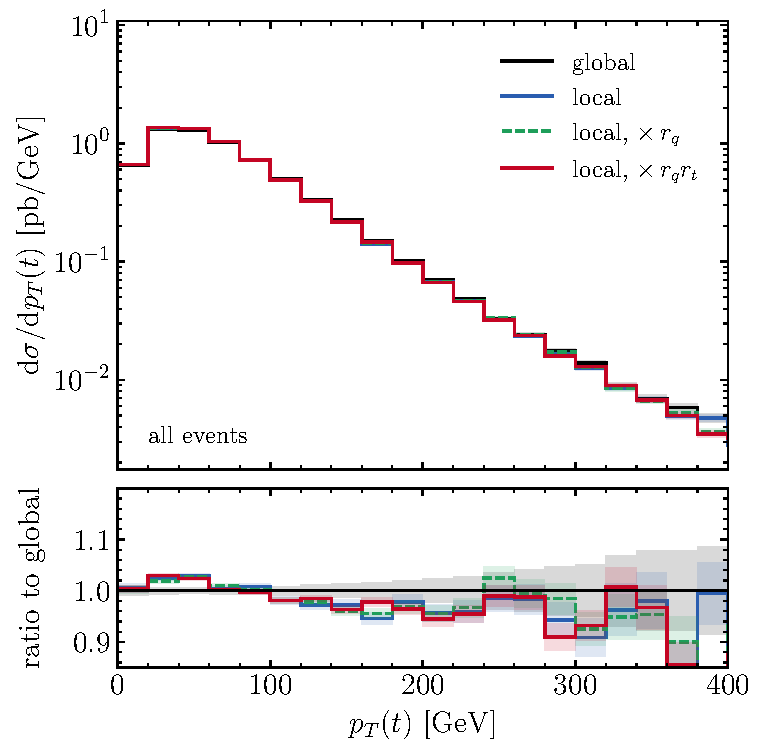
\includegraphics[width=0.49\textwidth]{figures/ptt_all.pdf}\hfill
  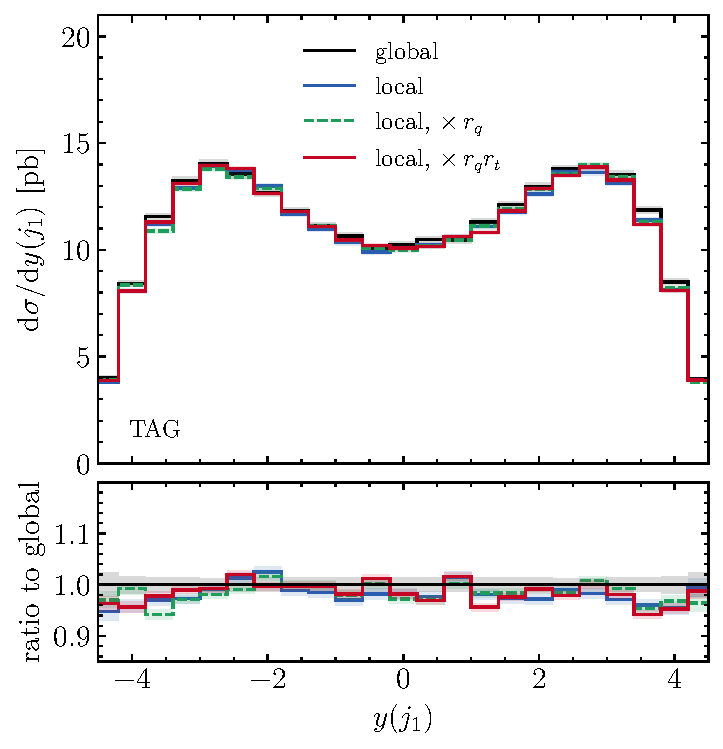
\includegraphics[width=0.49\textwidth]{figures/yj1_tag.pdf}
  \caption{Transverse momentum of the top quark for all events (left),
    and rapidity of the leading jet in the TAG selection (right). The
    lower panels show the ratios to the \glob prediction. The bands
    show the statistical uncertainties; in the lower panels, the
    coloured bands show the statistical uncertainties of the respective
    predictions divided by the \glob prediction, and the gray band
    shows the relative statistical uncertainty of the \glob
    prediction.}
  \label{fig:inclusive}
\end{figure}

Observables that are inclusive over additional radiation, such as
those of the top quark and the leading jet, are described at NLO
accuracy. Observables that require a second jet are described at LO
accuracy by the real-emission matrix elements, while a third and
further jets, as well as the regions of a small transverse momentum of
the top-quark--leading-jet system and of near back-to-back top quarks
and leading jets, are determined by the shower.

We start with observables that are described at NLO accuracy, in
figure~\ref{fig:inclusive}. The transverse momentum of the top quark
and the rapidity of the leading jet agree to within a few per cent
between the four predictions. The largest difference is in the tail of
the top-quark transverse momentum, which is about $7\%$ lower with
local recoil between 200 and $400\GeV$. This is consistent with the
fact that, with global recoil, the top quark also absorbs part of the
recoil of the ISR off the light-quark line, whereas with local recoil
this recoil is taken by the outgoing light quark only. Other
observables of the top quark and the leading jet, such as their
rapidity difference and invariant mass, agree to within about $3\%$
(not shown).

\begin{figure}[t]
  \centering
  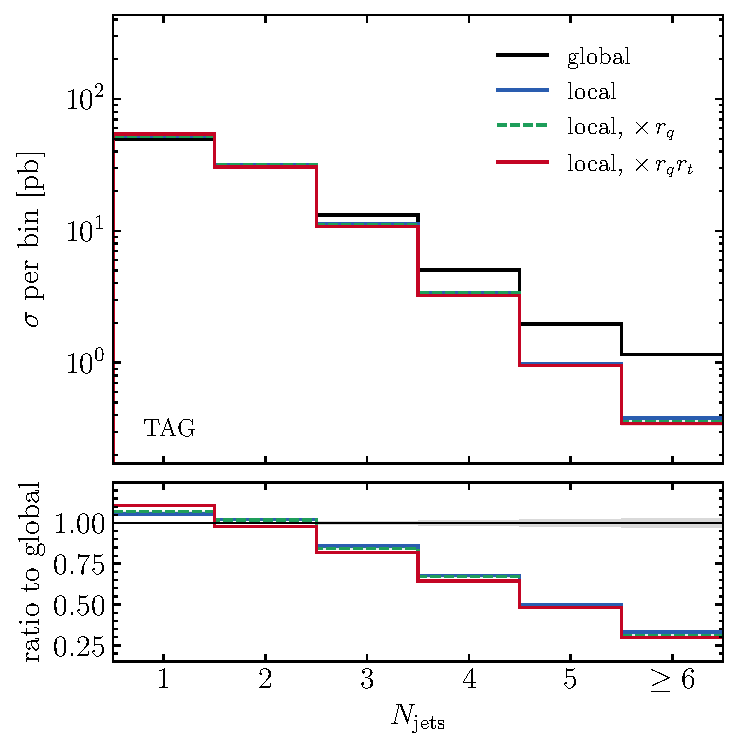
\includegraphics[width=0.49\textwidth]{figures/njets_tag.pdf}\hfill
  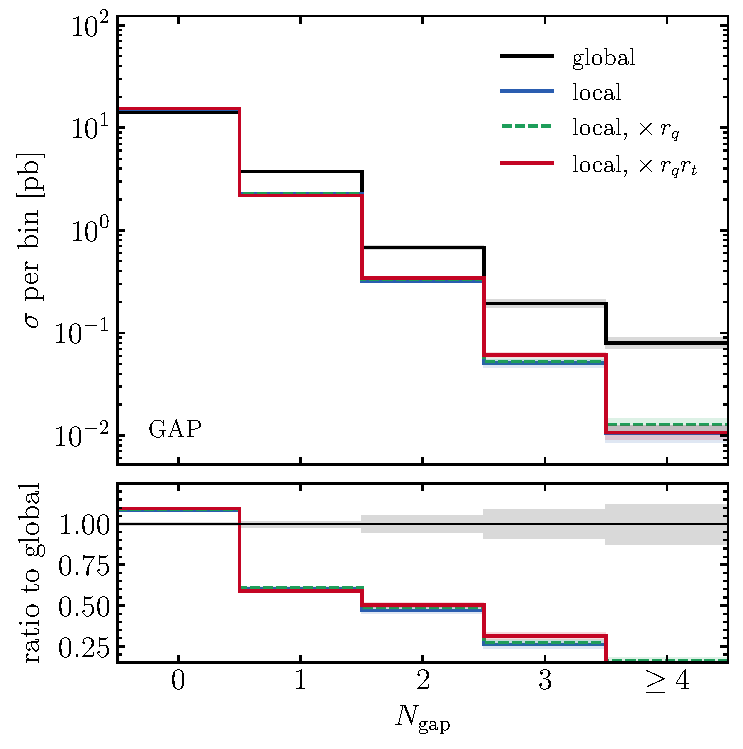
\includegraphics[width=0.49\textwidth]{figures/ngap_gap.pdf}
  \caption{Jet multiplicity in the TAG selection (left) and multiplicity
    of jets, other than the leading jet, in the rapidity interval
    between the top quark and the leading jet in the GAP selection
    (right). The last bins include the higher multiplicities. Lower
    panels and bands as in figure~\ref{fig:inclusive}.}
  \label{fig:multiplicities}
\end{figure}

The jet multiplicities are shown in figure~\ref{fig:multiplicities}.
With local recoil, the rate of events with two jets increases by $6$
to $9\%$, while those with more jets are strongly reduced: by $13$ to
$17\%$ for three jets, by about a third for four jets, and by
about a factor of three for six or more jets in the TAG selection. In
the GAP selection, the rates of events with one, two and three jets in
the rapidity gap are reduced by about $30\%$, $55\%$ and $70\%$,
respectively. Apart from the bins with one and two jets, which are
described at NLO and LO accuracy, respectively, these multiplicities
are determined by the shower, and the differences between the
predictions reflect the different shower recoil schemes. A suppression
by a factor of three for six or more jets thus shows the large shower
dependence of these rates, rather than a precise prediction for
them. With global recoil, the recoil of each ISR emission,
and of the first FSR emission, is distributed over the whole final
state, including the hard jets and the top quark. As in VBF Higgs
production~\cite{Jager:2020hkz}, this results in more radiation, in
particular in the central region.

\begin{figure}[t]
  \centering
  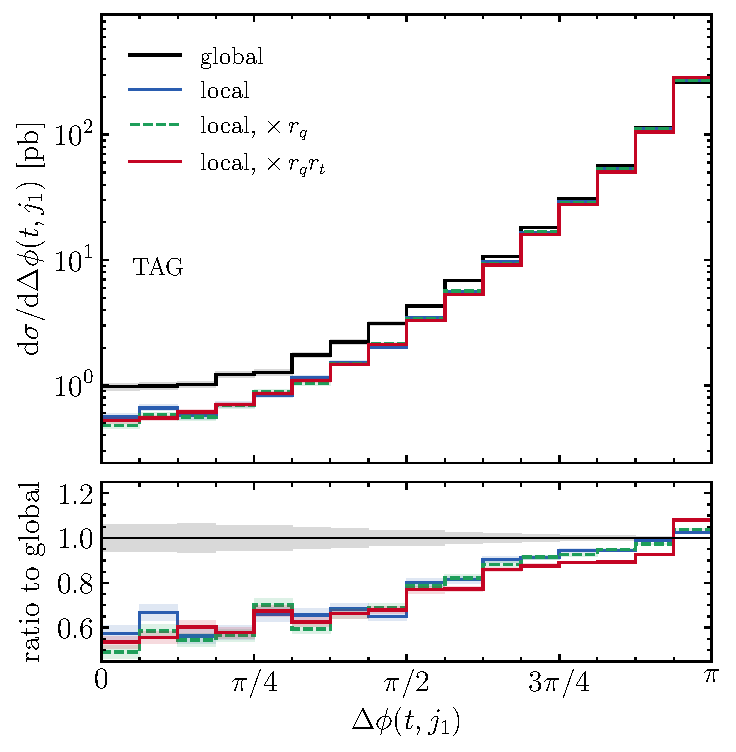
\includegraphics[width=0.49\textwidth]{figures/dphi_tag.pdf}\hfill
  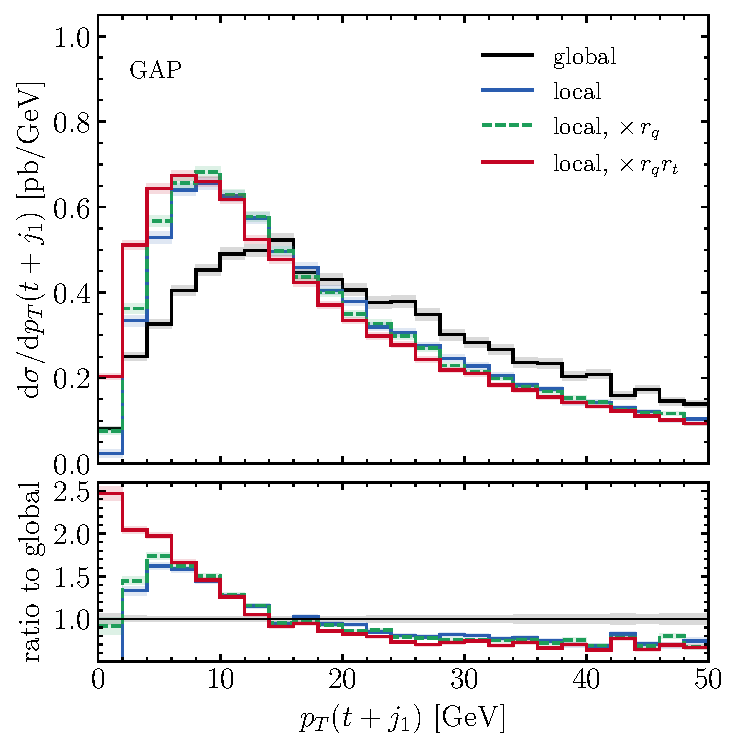
\includegraphics[width=0.49\textwidth]{figures/ptsys_gap.pdf}
  \caption{Azimuthal separation between the top quark and the leading
    jet in the TAG selection (left), and transverse momentum of the
    system of the top quark and the leading jet in the GAP selection
    (right). Lower panels and bands as in figure~\ref{fig:inclusive}.}
  \label{fig:recoil}
\end{figure}

The recoil of the top-quark--leading-jet system against additional
radiation is shown in figure~\ref{fig:recoil}. At the Born level, the
top quark and the leading jet are back to back. With local recoil, the
rate of configurations far from back to back is lower: by about $40\%$
for $\Delta\phi(t,j_1)<\pi/4$ and by about $25\%$ for $\pi/4<\Delta\phi(t,j_1)<\pi/2$
in the TAG selection, and by more in the GAP selection. With a single
additional parton, transverse-momentum conservation implies that for
$\Delta\phi(t,j_1)<\pi/2$ this parton is harder than the leading jet,
so that it must be outside the jet acceptance; this region is
therefore populated by multiple emissions or by radiation outside the
jet acceptance, and it is determined by the shower. Consistently,
the transverse momentum of the top-quark--leading-jet system is
smaller with local recoil, with $10$ to $17\%$ lower rates for
$\pT(t+j_1)>20\GeV$ in the GAP selection. At small values of
$\pT(t+j_1)$, below $5\GeV$, the local-recoil predictions differ among
themselves: the \locqt prediction is higher than the \locq one by
about $40\%$, both in the TAG and in the GAP selection. This region,
which contains between $6$ and $12\%$ of the cross section, is
sensitive to all soft radiation, including the shower cutoff and the
treatment of the bottom-quark mass in the shower, and the $r_t$
correction suppresses the soft radiation off the top quark in the
direction of its dead cone. In the GAP selection, the \loc prediction is lower than the
\locq one in this region, in particular in the first bin, where its
statistical uncertainty is large. Part of this difference may be due
to the mismatch of eq.~\eqref{eq:mismatch}, which affects soft and
collinear emissions only.

\begin{figure}[t]
  \centering
  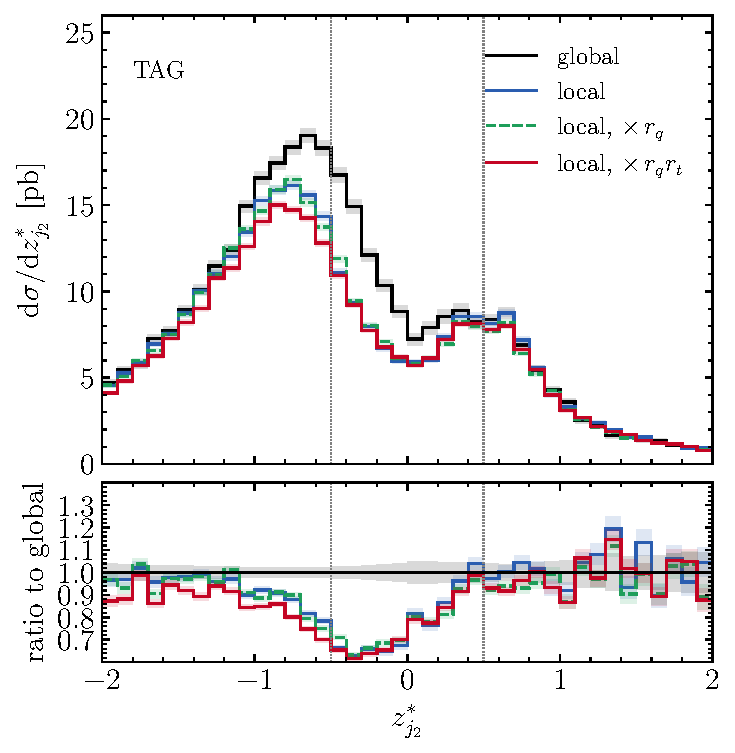
\includegraphics[width=0.49\textwidth]{figures/zstar_tag.pdf}\hfill
  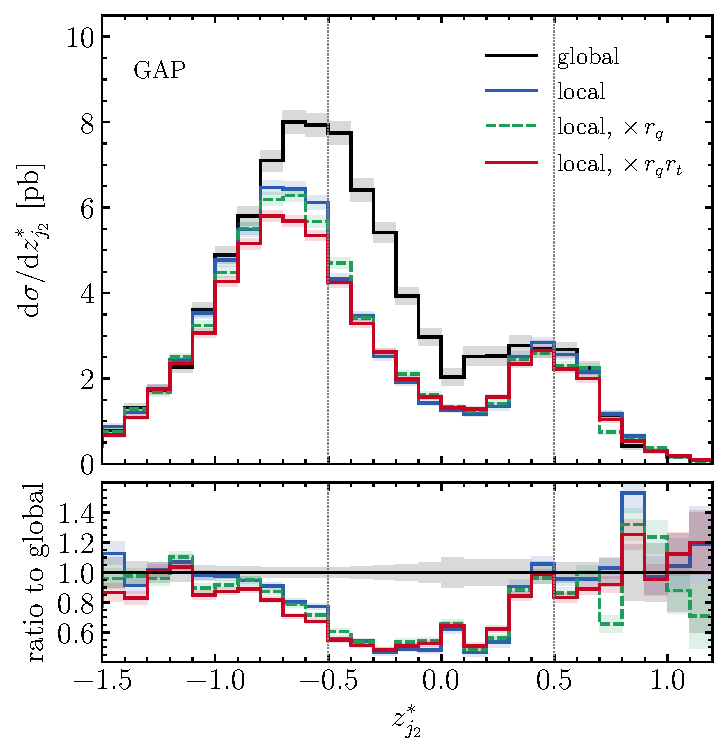
\includegraphics[width=0.49\textwidth]{figures/zstar_gap.pdf}
  \caption{Oriented Zeppenfeld variable of the second jet,
    eq.~\eqref{eq:zstar}, in the TAG (left) and GAP (right) selections,
    with $|y(j_1)-y(t)|>1$. The top quark is at $z^*=-1/2$ and the
    leading jet at $z^*=+1/2$, as indicated by the dotted lines.
    Lower panels and bands as in figure~\ref{fig:inclusive}.}
  \label{fig:zstar}
\end{figure}

The position of the second jet is shown in figure~\ref{fig:zstar}. The
second jet is mostly found close to the top quark, with a maximum just
outside the rapidity interval between the top quark and the leading
jet, and with a second maximum close to the leading jet. With local
recoil, the rate in the rapidity interval, $|z^*|<1/2$, is strongly
reduced, by about $25\%$ ($32\%$) in the half adjacent to the top
quark in the TAG (GAP) selection. This is qualitatively similar to
what has been observed in VBF Higgs
production~\cite{Jager:2020hkz,Hoche:2021mkv}. Outside the interval,
the differences are smaller. Close to the leading jet, $1/2<z^*<1$,
the \loc prediction is similar to (TAG) or about $10\%$ higher than
(GAP) the \glob one, whereas the \locq and \locqt predictions are
about $5$ to $10\%$ lower in both selections. To the extent that the
leading jet originates from the outgoing light quark, this is
consistent with the effect of the $r_q$ correction, which reduces the
hard-collinear radiation off this quark: in the unmodified shower, the
corresponding numerator, $2$ instead of $1+\zeta^2$, overestimates it.

\begin{figure}[t]
  \centering
  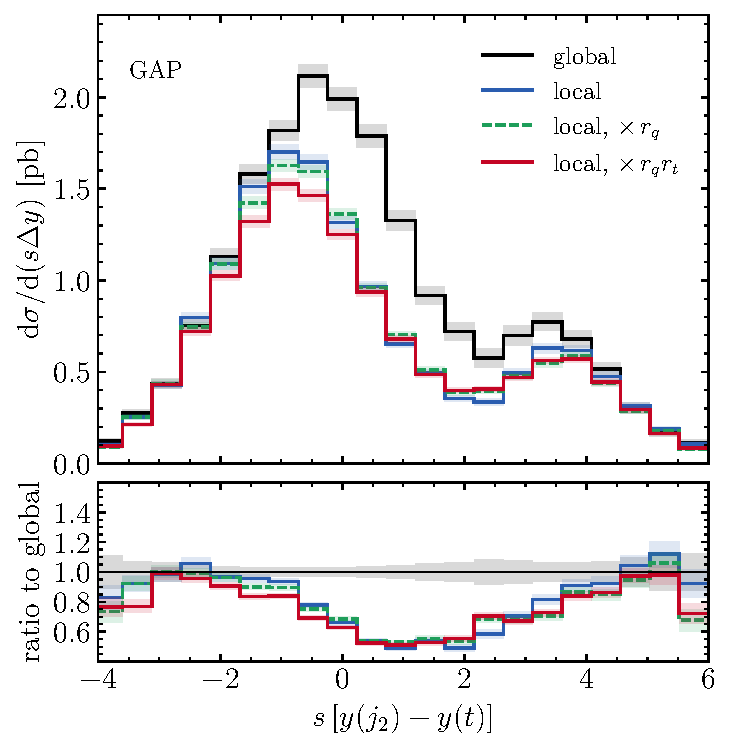
\includegraphics[width=0.49\textwidth]{figures/dyj2t_gap.pdf}\hfill
  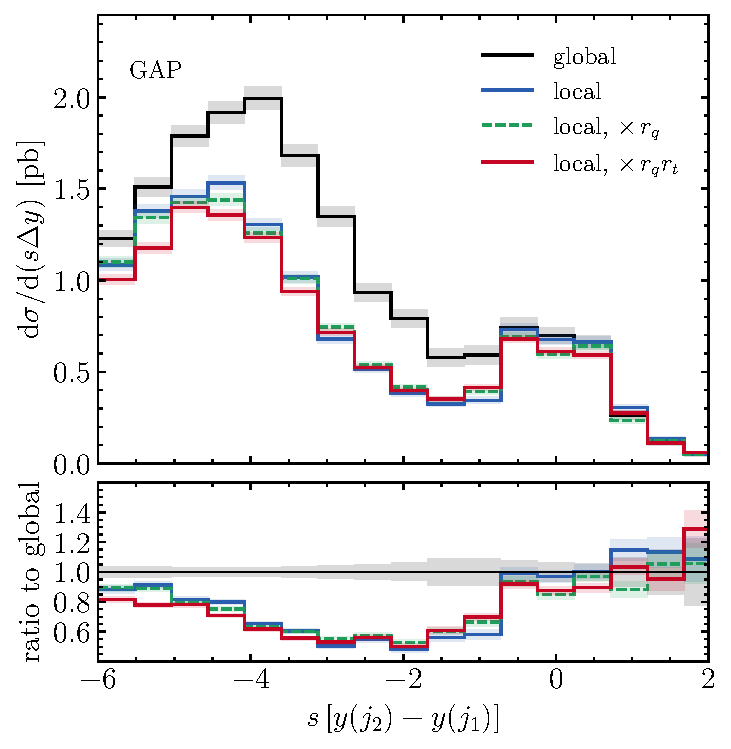
\includegraphics[width=0.49\textwidth]{figures/dyj2j1_gap.pdf}
  \caption{Oriented rapidity difference between the second jet and the
    top quark (left), and between the second jet and the leading jet
    (right), in the GAP selection. Negative values on the left
    (positive values on the right) correspond to the second jet outside
    the rapidity interval between the top quark and the leading jet,
    on the side of the top quark (leading jet). Lower panels and bands
    as in figure~\ref{fig:inclusive}.}
  \label{fig:dy}
\end{figure}

Figure~\ref{fig:dy} shows the rapidity of the second jet relative to
the top quark and to the leading jet in the GAP selection, in which
their rapidity difference is larger than three. The local recoil
reduces the rate of second jets in the rapidity gap by $30$ to $40\%$,
for rapidity distances between one and three from the top quark or
from the leading jet. Close to, and beyond, the top quark and the
leading jet, the differences between global and local recoil are
smaller. These distributions also indicate the effects of the two
kernel corrections. From the \loc to the \locq prediction, the rate of
second jets within one unit of rapidity beyond the leading jet
decreases by $17\%$, while the rate close to the top quark changes
little. Conversely, from the \locq to the \locqt prediction, the rate
of second jets within two units of rapidity beyond the top quark
decreases by about $7\%$, while the rate close to the leading jet
changes little. Note, however, that between these predictions also the
G-function prescription changes, from the profile $g_h(w)$ to
$g_h(\xi)$ and then to no G functions, so that these differences
cannot be attributed to the kernel corrections alone.
\todo{Controlled comparison with a common G-function prescription, or
  variations of the profiles, to separate the effects of the kernel
  corrections from those of the G functions.}
% Proposed runs: P in TODO_runs.txt and proposed_runs.csv. The runner
% run_g_variations.py forces PythiaLocalGProfile=1 for these new samples.

\begin{figure}[t]
  \centering
  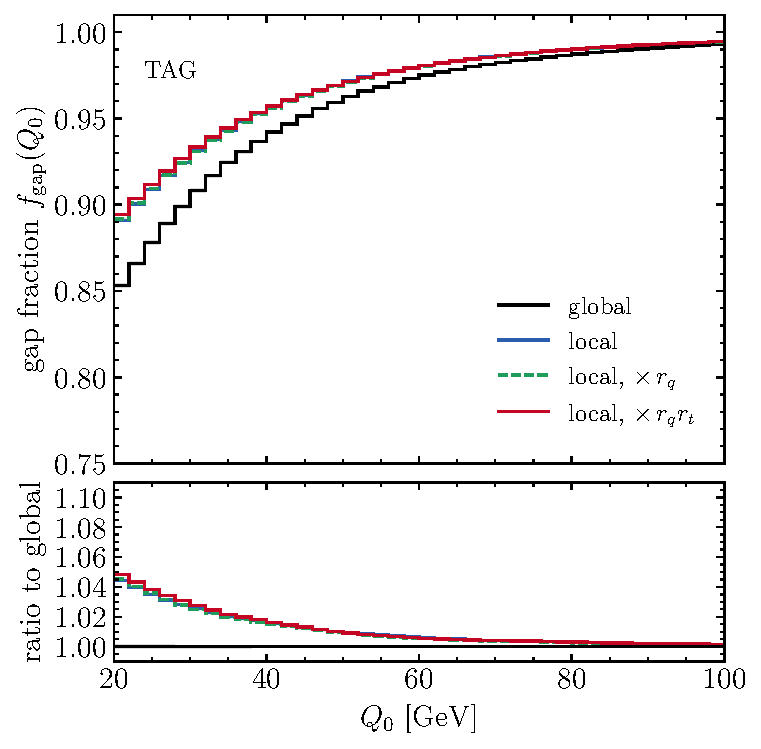
\includegraphics[width=0.49\textwidth]{figures/veto_tag.pdf}\hfill
  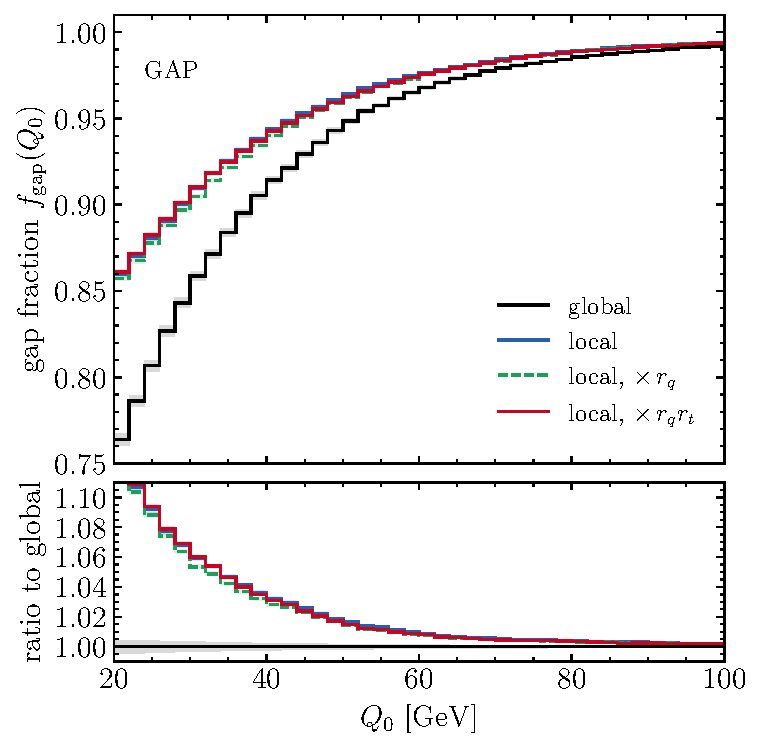
\includegraphics[width=0.49\textwidth]{figures/veto_gap.pdf}
  \caption{Gap fraction as a function of the veto scale $Q_0$, for the
    TAG (left) and GAP (right) selections, evaluated at
    $Q_0=21,23,\ldots,99\GeV$. The values at different $Q_0$ are
    statistically correlated. Lower panels and bands as in
    figure~\ref{fig:inclusive}.}
  \label{fig:veto}
\end{figure}

Finally, the gap fractions are shown in figure~\ref{fig:veto}. At
$Q_0=21\GeV$, the gap fraction increases from $0.857$ with global
recoil to between $0.890$ and $0.894$ with local recoil in the TAG
selection, and from $0.789$ to between $0.856$ and $0.861$ in the GAP
selection, i.e., by about seven percentage points. In other words, the
probability to find an additional jet with $\pT\ge21\GeV$ in the
rapidity gap of the GAP selection is reduced by about a third. Unlike
the rate of second jets in the gap, the gap fraction is sensitive to
any additional jet in the gap, not only to the second jet. The
difference decreases with $Q_0$: at
$Q_0=41\GeV$ ($61\GeV$), the gap fractions in the GAP selection are
$0.925$ ($0.968$) with global recoil and between $0.941$ and $0.945$
($0.976$) with local recoil. The three local-recoil predictions agree
with each other to within $0.6\%$ for all $Q_0$. Hence, for the gap
fraction, the effect of the recoil scheme is much larger than that of
the kernel corrections.


\section{Conclusions}
\label{sec:conclusions}

We have presented a proof of concept of \mcatnlo matching to \pythia
with local recoil, for $t$-channel single-top production with a stable
top quark in the five-flavour scheme. The local recoil map of the IF
dipoles of \pythia has been implemented in the FKS phase-space
generation of \mgamc, in both FKS sectors of each dipole, and the MC
counterterms are given by the first-emission density of the IF
dipoles, which is divided over the two sectors.

The first-emission expansion of the unmodified shower fails to
reproduce two limits of the real-emission matrix elements: the
hard-collinear limit of radiation off the outgoing light quark, and
the soft limit of radiation off the massive top quark, which lacks
the dead cone. Without further measures, the \mcatnlo short-distance
cross sections would then be divergent. We have considered two ways to
address this. With the unmodified \pythia shower, the MC counterterms
are replaced by the FKS soft and collinear counterterms in a small
region around these limits, through G functions. Alternatively, the
IF kernel of the shower can be corrected, with a numerator
$z^2+\zeta^2$ instead of $1+z^2$ and a suppression factor $r_t$ for
radiation off the top quark in its IF dipole with an incoming quark.
Both corrections are bounded by one and are applied in the veto step
of the shower. With both, the shower has the correct soft and
collinear limits for this process, for massless incoming quarks, and
the MC counterterms need no G functions.

Compared to the default global recoil, the three local-recoil
predictions agree to within a few per cent for most observables that
are described at NLO accuracy. They predict, however, substantially
less radiation in the rapidity region between the top quark and the
leading jet. The rate of events with a second jet in this region is
reduced by about $20$ to $30\%$, the probability of an additional jet
above $21\GeV$ in the rapidity gap by about a third, and the rate of
events with many jets by up to a factor of three. This is
qualitatively similar to what has been found in VBF Higgs production.
The kernel corrections have smaller, localised effects: the $r_q$
correction reduces the radiation close to the leading jet, and the
$r_t$ correction the radiation close to the top quark, although these
effects cannot yet be fully separated from those of the G functions.
These numerical results hold for the shower setup used here, and they
are not accompanied by an assessment of the theoretical
uncertainties. In addition, the local-recoil samples have fewer
negative weights, with fractions of $26\%$, $23\%$ and $20\%$,
compared to $30\%$ with global recoil, so that, for the total cross
section, the \locqt prediction requires about half the number of
events for the same statistical precision.

The present implementation is restricted to Born processes with two
massless incoming quarks, one massive and one massless outgoing quark,
and two IF colour connections, and it fails explicitly for other
processes. We have not included the top-quark decay, hadronisation
and multiple interactions, nor theoretical uncertainties, such as scale,
PDF and matching uncertainties; in particular, the dependence on the
G-function width has only been checked for inclusive rates. The two
kernel corrections are modifications of \pythia that are not part of
the public code, and their effects on other processes, as well as the
logarithmic accuracy of the modified shower, remain to be studied.
Natural next steps are the extension to other processes with IF
dipoles only, such as VBF and vector-boson scattering, the inclusion of
the top-quark decay, which requires a consistent treatment of the
resonance in the matching~\cite{Jezo:2015aia} and for which
NLO+PS generators with off-shell effects
exist~\cite{Frederix:2016rdc,vanBeekveld:2026mjv}, and the extension to
initial-initial and final-final dipoles, which would make \mcatnlo
matching with local recoil available for general processes. Although
the GAP selection used here is a diagnostic rather than an experimental
fiducial region, the size of the effects that we observe suggests that
the recoil scheme should be considered in any assessment of the
uncertainties of NLO+PS predictions for $t$-channel single-top
production.

Our implementation extends \mgamc~3.8.0 and uses
\textsc{Pythia}~8.318 for the shower. This development version
contains the local FKS maps, the matching counterterms and the
parton-level analysis. The two shower corrections are supplied as
separate, optional source patches, with both switches off by default;
the corrected predictions use private builds of the shower. The
unmodified build is retained for the \glob and \loc predictions.
% Author action before publication: add the public source archive/DOI and
% immutable revision identifiers. No public release location is recorded
% in the implementation used for this study.

% \acknowledgments


\appendix

\section{Phase-space parametrisation in the initial-state sector}
\label{app:phasespace}

In this appendix, we give the relation between the variables
$(w,y,\varphi)$ used to generate the radiation in the initial-state
FKS sector and the FKS energy fraction $\xi$. Let the emitting
incoming parton move in the direction $\eta=\pm1$ along the beam axis,
and let $\hat s_{\mathrm{B}}=4e^2$ be the partonic centre-of-mass
energy squared of the Born configuration. In the Born centre-of-mass
frame, we denote the momentum of the colour partner by $f=\tilde p_f$,
with light-cone component $f_-=f^0-\eta f^3$, so that $D=2ef_-$. The
direction of the gluon in the partonic centre-of-mass frame of the
real-emission configuration is
\begin{equation}
  n=\left(1,\sqrt{1-y^2}\cos\varphi,\sqrt{1-y^2}\sin\varphi,\eta\,y\right).
  \label{eq:gluondirection}
\end{equation}
The two frames are related by a longitudinal boost with rapidity
$\frac{1}{2}\log\lambda$, where $\lambda=1/z=1/(1-w)$. With
\begin{align}
  A&=f_-(1+y)+2e(1-y)\,,\qquad
  B_\varphi=2\left(f^1\cos\varphi+f^2\sin\varphi\right)\sqrt{1-y^2}\,,\qquad
  T_0=2\,f\cdot n\,,\nonumber\\
  T&=T_0+(\lambda-1)\left(A-\frac{B_\varphi}{\sqrt\lambda+1}\right),
  \label{eq:Tdef}
\end{align}
where $f\cdot n$ is evaluated with the components of $f$ in the Born
and those of $n$ in the real-emission frame, the energy fraction of
the gluon in the real-emission frame is
\begin{equation}
  \xi=\frac{2E_k}{\sqrt{\hat s_{\mathrm{R}}}}=\frac{2f_-\lambda\,w}{T}\,.
  \label{eq:xi}
\end{equation}
In the collinear limit of the gluon and the incoming parton, $y\to1$,
one has $T=2\lambda f_-$ and therefore $\xi=w$. In the soft limit,
$\xi=a\,w+\order{w^2}$ with $a=2f_-/T_0$, which enters the finite soft
term of section~\ref{sec:phasespace}. The phase-space measure of
eq.~\eqref{eq:measure} becomes
\begin{equation}
  \dd x_a^{\mathrm{R}}\,\dd\PhiR=\dd x_a^{\mathrm{B}}\,\dd\PhiB\,
  \frac{\hat s_{\mathrm{R}}}{(4\pi)^3}\,\xi\,\frac{2f_-\lambda^2}{T}\,
  \dd w\,\dd y\,\dd\varphi\,,
  \label{eq:measurexi}
\end{equation}
where we have factored out $\xi$, as is customary in the FKS
parametrisation. The real-emission contribution uses the physical
$\xi$ of eq.~\eqref{eq:xi}, while the soft counterterm is the
coefficient of $\dd w/w$.

To evaluate the soft limits of the contributions to an $\clS$ event at
the same configuration (see section~\ref{sec:phasespace}), we generate
the direction of the soft gluon once, in the Born centre-of-mass frame,
and transform it to the frame of each FKS sector, including the
corresponding Jacobian. The physical energies of the soft gluon are
matched as well. Let $r$ be the variable in the unit interval from
which the gluon energy is generated in a common parametrisation, and
$r'$ the one of an FKS sector, with $\dd E/\dd(r^2)$ in the soft limit
larger by a factor $c>0$ for the latter. We use the bijection of the
unit interval
\begin{equation}
  r'=\frac{r}{\sqrt{c\,(1-r^2)+r^2}}\,,\qquad
  \frac{\dd r'}{\dd r}=\frac{c}{\left[c\,(1-r^2)+r^2\right]^{3/2}}\,,
  \label{eq:commonsoft}
\end{equation}
which matches the soft energies, $r'^2\simeq r^2/c$ for $r\to0$, and
removes the finite remainder that would arise from different soft
slopes. The $\clH$ events retain the variables of their own FKS sector.


\section{Implementation of the kernel corrections in Pythia8}
\label{app:pythia}

\begin{table}[t]
  \centering
  \begin{tabular}{@{}ll@{}}
    \toprule
    This paper & \pythia (\code{SimpleSpaceShower.cc})\\
    \midrule
    $z$ & \code{z}, the backward-evolution momentum fraction\\
    $Q^2$ & \code{Q2}, the space-like virtuality $-(p_a-k)^2$\\
    $\zeta$ & $z_1=1-zQ^2/(m_{\mathrm{dip}}^2-m_f^2)$\\
    $D$ & \code{m2ColPair - m2ColPartner}, i.e., $m_{\mathrm{dip}}^2-m_f^2$\\
    $wQ^2$ & \code{pT2}, the evolution variable $p^2_{\perp\mathrm{evol}}$\\
    $\kt^2$ & \code{pT2corr}, the transverse momentum of the emission\\
    \bottomrule
  \end{tabular}
  \caption{Correspondence between the variables of this paper and those
    of the IF branchings with \code{SpaceShower:dipoleRecoil = on} in
    \textsc{Pythia}~8.318.}
  \label{tab:pythiavariables}
\end{table}

Both corrections of section~\ref{sec:patches} are implemented as
additional factors of the acceptance weight of a trial branching in
the backward evolution, in \code{SimpleSpaceShower.cc}, before the
branching is accepted. The correspondence of the variables is given in
table~\ref{tab:pythiavariables}. The corrections are controlled by two
new flags, both switched off by default,
\begin{center}
  \code{SpaceShower:IFquarkCollinearCorrection = on}\,,\qquad
  \code{SpaceShower:IFtopSoftCorrection = on}\,,
\end{center}
where we use the second only together with the first. The first
multiplies the weight
by $r_q=(z^2+z_1^2)/(1+z^2)$ for a $q\to qg$ branching of an incoming
quark whose colour partner is an outgoing quark or antiquark. The
second multiplies the weight, in addition, by
\begin{center}
  \code{double z1 = 1. - z * Q2 / (m2ColPair - m2ColPartner);}\\
  \code{wt *= pT2corr / (pT2 * z1);}
\end{center}
which is $r_t=\kt^2/(wQ^2\zeta)$ of eq.~\eqref{eq:rt}, for a branching
in which the incoming quark keeps its flavour and emits a gluon, and in
which the colour partner is an outgoing top quark or antiquark. The
recoil kinematics, the masses, the thresholds and all other
branchings are unchanged. In \mgamc, the corresponding MC counterterms
are selected with two flags in \code{FKS\_params.dat}, which also set
the corresponding \pythia flags in the shower steering file.

\bibliographystyle{JHEP}
\bibliography{references}

\end{document}
